\documentclass[12pt]{article}

% Load packages
\usepackage{url}  % Formatting web addresses
\usepackage{ifthen}  % Conditional
\usepackage{multicol}   %Columns
\usepackage[utf8]{inputenc} %unicode support
\usepackage{amsmath}
\usepackage{amssymb}
\usepackage{epsfig}
\usepackage{epstopdf}
\usepackage{graphicx}
\usepackage{cite}
\usepackage{lastpage,fancyhdr,graphicx}
\usepackage{mathtools}
\usepackage[margin=0.1pt,font=footnotesize,labelfont=bf]{caption}
\usepackage{setspace}
%\usepackage{longtable}
\usepackage{colortbl}
%\usepackage{palatino,lettrine}
%\usepackage{times}
%\usepackage[applemac]{inputenc} %applemac support if unicode package fails
%\usepackage[latin1]{inputenc} %UNIX support if unicode package fails
\usepackage[wide]{sidecap}
%\usepackage[authoryear,round,comma,sort&compress]{natbib}
\usepackage[square,sort,comma,numbers,sort&compress]{natbib}
%\usepackage[authoryear,round]{natbib}
\usepackage{supertabular}
\usepackage{simplemargins}
\usepackage{fullpage}
\usepackage{comment}
\usepackage{lineno}
%\usepackage{chicago}
\usepackage{textcomp}
\usepackage{multirow}
\usepackage{amsmath}
\usepackage{color}
\usepackage{booktabs}
\usepackage{xfrac}
\setlength\heavyrulewidth{0.4ex}
\setlength\lightrulewidth{0.25ex}
%\usepackage{textgreek}
%\usepackage[linesnumbered,lined,boxed,commentsnumbered]{algorithm2e}
\DeclareMathOperator*{\argmin}{\arg\!\min}

%\usepackage{algorithm2e}
%\usepackage{algpseudocode}
%\usepackage[space]{cite}
\urlstyle{rm}
\hyphenation{dec-ades} %Latex does not know how to hyphenate this by default, so we add it to the list
\def\wl{\par \vspace{\baselineskip}}

%\textwidth = 6.50 in
%\textheight = 9.5 in
%\oddsidemargin =  0.0 in
%\evensidemargin = 0.0 in
%\topmargin = -0.50 in
%\headheight = 0.0 in
%\headsep = 0.25 in
%\parskip = 0.15in
%\linespread{1.75}
\doublespace

%\bibliographystyle{chicago}
\bibliographystyle{plos2015}

\makeatletter
\renewcommand\subsection{\@startsection
	{subsection}{2}{0mm}
	{-0.05in}
	{-0.5\baselineskip}
	{\normalfont\normalsize\bfseries}}
\renewcommand\subsubsection{\@startsection
	{subsubsection}{2}{0mm}
	{-0.05in}
	{-0.5\baselineskip}
	{\normalfont\normalsize\itshape}}
\renewcommand\section{\@startsection
	{subsection}{2}{0mm}
	{-0.2in}
	{0.05\baselineskip}
	{\normalfont\large\bfseries}}
\renewcommand\paragraph{\@startsection
	{paragraph}{2}{0mm}
	{-0.05in}
	{-0.5\baselineskip}
	{\normalfont\normalsize\itshape}}
\makeatother

%Review style settings
%\newenvironment{bmcformat}{\begin{raggedright}\baselineskip20pt\sloppy\setboolean{publ}{false}}{\end{raggedright}\baselineskip20pt\sloppy}

%Publication style settings

% Single space'd bib -
\setlength\bibsep{0pt}

\renewcommand{\rmdefault}{phv}\renewcommand{\sfdefault}{phv}
\newcommand{\norm}[1]{\left\lVert#1\right\rVert}

% Change the number format in the ref list -
\renewcommand{\bibnumfmt}[1]{#1.}

% Change Figure to Fig.
\renewcommand{\figurename}{Fig.}

% Begin ...
\begin{document}
\begin{titlepage}
{\par\centering\textbf{\Large {Toward a Genome Scale Dynamic Model of Cell-Free Protein Synthesis in \emph{Escherichia~coli}}}}
\vspace{0.05in}
{\par \centering \large{Nicholas Horvath, Michael Vilkhovoy, Joseph Wayman, Kara Calhoun$^{1}$, James Swartz$^{1}$ and Jeffrey D. Varner$^{*}$}}
\vspace{0.10in}
{\par \centering {Robert Frederick Smith School of Chemical and Biomolecular Engineering}}
{\par \centering {Cornell University, Ithaca NY 14853}}
\vspace{0.1in}
{\par \centering {$^{1}$School of Chemical Engineering}}
{\par \centering {Stanford University, Stanford, CA 94305}}
{\par \centering \textbf{Running Title:}~Dynamic modeling of cell-free protein synthesis}
\vspace{0.1in}
{\par \centering \textbf{To be submitted:}~\emph{Scientific~Reports}}
\vspace{0.5in}
{\par \centering $^{*}$Corresponding author:}
{\par \centering Jeffrey D. Varner,}
{\par \centering Professor, Robert Frederick Smith School of Chemical and Biomolecular Engineering,}
{\par \centering 244 Olin Hall, Cornell University, Ithaca NY, 14853}
{\par \centering Email: jdv27@cornell.edu}
{\par \centering Phone: (607) 255 - 4258}
{\par \centering Fax: (607) 255 - 9166}
\end{titlepage}
\date{}
\thispagestyle{empty}
\pagebreak
%%%%%%%%%%%%%%%%%%%%%%%%%%%%%%%%%%%%%%%%%%%%%%%%%%%%%%%%%%%%%%%%%%%%%%%%%%%%%%%%%%%%%%%%%%%%%%%%%%%%%%%%%%%
%%%%%%%%%%%%%%%%%%%%%%%%%%%%%%%%%%%%%%%%%%%%%%%%%%%%%%%%%%%%%%%%%%%%%%%%%%%%%%%%%%%%%%%%%%%%%%%%%%%%%%%%%%%
\section*{Abstract}
Cell-free protein expression systems have become widely used in systems and synthetic biology.
In this study, we developed an ensemble of dynamic \textit{E. coli} cell-free protein synthesis (CFPS) models.
Model parameters were estimated from a training dataset for the cell-free production of a protein product, chloramphenicol acetyltransferase (CAT).
The dataset consisted of measurements of glucose, organic acids, energy species, amino acids, and CAT.
The ensemble accurately predicted these measurements, especially those of the central carbon metabolism.
We then used the trained model to evaluate the optimality of protein production.
CAT was produced with a carbon yield of 7\% and an energy efficiency of 5\%, suggesting that the process could be further optimized.
Reaction group knockouts showed that protein productivity and the metabolism as a whole depend most on oxidative phosphorylation and glycolysis and gluconeogenesis.
Amino acid biosynthesis is also important for productivity, while the overflow metabolism and TCA cycle affect the overall system state.
In addition, CAT production was robust to allosteric control, as was most of the network, with the exception of the organic acids in central carbon metabolism.
This study is the first to use kinetic modeling to predict dynamic protein production in a cell-free \textit{E. coli} system, and should provide a foundation for genome scale, dynamic modeling of cell-free \textit{E. coli} protein synthesis.

\vspace{0.1in}
{\noindent \textbf{Keywords:}~Biochemical engineering, systems biology, \textit{E. coli}, cell-free protein synthesis, kinetic modeling}

\pagebreak

\setcounter{page}{1}

%In this study, we present a framework for dynamic, cell-free metabolic modeling, integrating a simple logical description of regulation with traditional enzyme kinetics.
%Using this framework, we have constructed an ensemble of models for production of chloramphenicol acetyltransferase in a cell-free \textit{E. coli} system.
%Our ensemble fits measurements of glucose, chloramphenicol acetyltransferase, organic acids, and energy species, but fails to capture much of the amino acid dynamics in the dataset.

% Uncomment in production -
\linenumbers

% Interestingly, many of the challenges confronting genome scale kinetic modeling can potentially be overcome in a cell-free system.
% For example, there is no complex transcriptional regulation to consider, transient metabolic measurements are easier to obtain, and we no longer have to consider cell growth.
% Thus, cell-free operation holds several significant advantages for model development, identification and validation. Theoretically, genome scale cell-free kinetic models may be possible for industrially important organisms,
% such as \textit{E. coli} or \textit{B.~subtilis}, if a simple, tractable framework for integrating allosteric regulation with enzyme kinetics can be formulated.
% Conversely, highly abstracted kinetic frameworks, such as the cybernetic framework, represented a paradigm shift, viewing cells as growth-optimizing strategists \citep{1985_dhurjati_ramkrishna_tsao_BiotechBioeng}.
% Cybernetic models have been highly successful at predicting metabolic choice behavior, e.g., diauxie behavior \citep{1986_kompala_ramkrishna_tsao_BiotechBioeng}, steady-state multiplicity \citep{2012_kim_ramkrishna_BiotechProg}, as well as the cellular response to metabolic engineering modifications \citep{1999_varner_ramkrishna_MetaEng}.
% Unfortunately, traditional, fully structured cybernetic models also suffer from an identifiability challenge, as both the kinetic parameters and an abstracted model of cellular objectives must be estimated simultaneously.
% However, recent cybernetic formulations from Ramkrishna and colleagues have successfully treated this identifiability challenge through elementary mode reduction~\cite{2009_song_ramkrishna_BiotechBioeng,Song:2011aa}.

\section*{Introduction}

Cell-free systems offer many advantages for the study, manipulation and modeling of metabolism compared to \textit{in vivo} processes.
Central amongst these is direct access to metabolites and the biosynthetic machinery without the interference of a cell wall, or complications associated with cell growth.
This allows us to interrogate the chemical environment while the biosynthetic machinery is operating, potentially at a fine time resolution.
Cell-free protein synthesis (CFPS) systems are arguably the most prominent examples of cell-free systems used today \citep{Jewett:2008aa}.
However, CFPS is not new; CFPS in crude \textit{E.~coli} extracts has been used since the 1960s to explore fundamentally important biological mechanisms \citep{MATTHAEI:1961aa,NIRENBERG:1961aa}.
Today, cell-free systems are used in a variety of applications ranging from therapeutic protein production \citep{Lu:2014aa} to synthetic biology \citep{Hodgman:2012aa,Pardee:2016aa}.
However, if CFPS is to become a mainstream technology for applications such as point of care manufacturing, we must first understand the performance limits of these systems.
One tool we can use to achieve this understanding is mathematical modeling.

Mathematical modeling has long contributed to our understanding of metabolism.
Decades before the genomics revolution, mechanistically structured metabolic models arose from the desire to predict microbial phenotypes resulting from changes in intracellular or extracellular states \citep{1976_fredrickson_BiotechBioeng}.
The single cell \textit{E. coli} models of Shuler and coworkers pioneered the construction of large-scale, dynamic metabolic models that incorporated multiple regulated catabolic and anabolic pathways constrained by experimentally determined kinetic parameters \citep{1984_domach_shuler_BiotechBioeng_01}.
Shuler and coworkers generated many single cell kinetic models, including single cell models of eukaryotes \citep{1989_steinmeyer_shuler_ChemEngSci,1992_wu_shuler_AnnNYAcadSci}, minimal cell architectures \citep{2004_castellanos_shuler_PNAS}, as well as DNA sequence based whole-cell models of \textit{E. coli} \citep{2008_atlas_shuler_IETSysBio}.
%In the post genomics world, large-scale stoichiometric reconstructions of microbial metabolism popularized by techniques such as flux balance analysis (FBA) have become a standard approach \citep{2012_lewis_palsson_NatRevMicrobio}.
%Since the first genome scale stoichiometric model of \textit{E. coli} developed by Edwards and Palsson \citep{2000_edwards_palsson_PNAS}, well over 100 organisms including industrially important prokaryotes are now available \citep{2009_feist_palsson_NatRevMicrobio,Feist:2007aa,Oh:2007aa}.
%Stoichiometric models rely on a pseudo-steady-state assumption to reduce unidentifiable genome scale kinetic models to an underdetermined linear algebraic system, which can be solved efficiently even for large systems.
%Traditionally, stoichiometric models have also neglected explicit descriptions of metabolic regulation and control mechanisms, instead opting to describe the choice of pathways by prescribing an objective function on metabolism. Interestingly, similar to early cybernetic models, the most common metabolic objective function has been the optimization of biomass formation \citep{2002_ibarra_edwards_palsson_Nat}, although other metabolic objectives have also been estimated \citep{2007_schuetz_sauer_MolSysBio}.
%Recent advances in constraint-based modeling have overcome the early shortcomings of the platform, including capturing metabolic regulation and control \citep{2013_hyduke_lewis_palsson_MolBioSys}.
%Thus, modern constraint-based approaches have proven extremely useful in the discovery of metabolic engineering strategies and represent the state of the art in metabolic modeling \citep{2013_mccloskey_palsson_feist_MolSysBio, 2012_zomorrodi_maranas_MetaEng}.
However, cell-free genome scale kinetic models of industrially important organisms such as \textit{E. coli} have yet to be constructed.

In this study, we developed an ensemble of kinetic cell-free protein synthesis (CFPS) models using dynamic metabolite measurements in an \textit{E. coli} cell-free extract.
Model parameters were estimated from measurements of glucose, organic acids, energy species, amino acids, and the protein product, chloramphenicol acetyltransferase (CAT).
The parameter estimation problem was constrained by characteristic values for model parameters from literature.
The ensemble of parameter sets described the training data with a median cost that was more than two orders of magnitude smaller than random sets constructed using the literature parameter constraints.
We then used the ensemble of kinetic models to analyze the optimality of the CFPS system, and the pathways most important to CAT production.
We calculated that CAT was produced with a carbon yield of 7\% and an energy efficiency of 5\%, suggesting that much of the resources for protein synthesis were diverted to non-productive pathways.
By knocking out metabolic enzymes in groups, we showed that the system metabolism and protein production depend most on oxidative phosphorylation and glycolysis\slash gluconeogenesis.
%By knocking out metabolic enzymes in groups, we showed that CAT productivity depends most on oxidative phosphorylation, glycolysis\slash gluconeogenesis, and certain amino acid synthesis reactions, while the system state is most sensitive to glycolysis\slash gluconeogenesis, oxidative phosphorylation, the overflow metabolism, and the TCA cycle reactions.
%First, sensitivity analysis of the dynamic model suggested that CAT production was most sensitive to CAT synthesis parameters, as well as reactions in oxidative phosphorylation and pyruvate consumption.
%Sensitivity analysis also showed that the system as a whole was most sensitive to these same parts of the network and glucose consumption.
%CAT production and other metabolites, specifically organic acid intermediates such as pyruvate, were sensitive to the presence of allosteric control mechanisms.
Taken together, we have integrated traditional kinetics with a logical rule-based description of allosteric control to simulate a comprehensive CFPS dataset.
This study provides a foundation for genome scale, dynamic modeling of cell-free \textit{E. coli} protein synthesis.

\clearpage

\section*{Results}

The cell-free \textit{E.~coli} metabolic network was constructed by removing growth associated reactions from the \textit{i}AF1260 reconstruction of K-12 MG1655 \textit{E.~coli} \cite{Feist:2007aa}, and by adding reactions describing chloramphenicol acetyltransferase (CAT) biosynthesis, a model protein for which there exists a comprehensive training dataset \cite{2005_calhoun_BiotechnologyProgress}.
In addition, reactions that were knocked out from the cell extract preparation were removed from the network ($\Delta$speA, $\Delta$tnaA, $\Delta$sdaA, $\Delta$sdaB, $\Delta$gshA, $\Delta$tonA, $\Delta$endA).
The CFPS model equations were formulated using the hybrid cell-free modeling framework of Wayman et al. \cite{pr3010138}.
An initial ensemble of model parameter sets (N $>$ 30,000) was estimated from measurements of glucose, CAT, organic acids (pyruvate, lactate, acetate, succinate, malate), energy species (A(x)P, G(x)P, C(x)P, U(x)P), and 18 of the 20 proteinogenic amino acids using a constrained Markov Chain Monte Carlo (MCMC) approach.
%The MCMC algorithm minimized the error between the training data and model simulations starting from an initial parameter set assembled from literature and inspection.
A final ensemble of parameter sets (N $=$ 100) was constructed by selecting the sets with the lowest errors, the lowest of which was defined as the best-fit set.
Parameter sets in the final ensemble had a mean Pearson correlation coefficient of 0.77; thus, an accurate yet diverse ensemble was created.

The ensemble of kinetic CFPS models captured the time evolution of CAT biosynthesis.
%(Fig.~\ref{fig:Carbon} - \ref{fig:Amino}).
Central carbon metabolites (Fig.~\ref{fig:Carbon}, top), energy species (Fig.~\ref{fig:Energy}), and amino acids (Fig.~\ref{fig:Amino}) were captured by the ensemble and the best-fit set.
The constrained MCMC approach estimated parameter sets with a median error more than two orders of magnitude less than random parameter sets generated within the same parameter bounds (Fig.~\ref{fig:BoxPlot}); thus, we have confidence in the predictive capability of the estimated parameters.
The model captured the biphasic CAT production: during the first hour glucose powers production, and CAT is produced at 10 $\mu$M/h; subsequently, pyruvate and lactate reserves are consumed to power metabolism, and CAT is produced less efficiently at 3 $\mu$M/h.
%Allosteric control was important to biphasic CAT production; without control, the CAT production rate increased and then ceased after 1.5 h (Fig.~\ref{fig:Carbon}, bottom).
%In addition, acetate no longer accumulated after 1.5 hours, in the absence of allosteric control.
%Interestingly, the simulated malate abundance tracked the experimental measurements during the glucose consumption phase, but increased sharply during the pyruvate consumption phase, without allosteric control.
Allosteric control was important to central carbon metabolism, especially pyruvate, acetate, and succinate (Fig.~\ref{fig:Carbon}, bottom).
The difference between the allosteric control and no-control cases is mostly seen in the second phase of CAT production, after glucose is exhausted.
Specifically, there is an increase in the consumption of pyruvate, succinate, and malate, as well as the accumulation of acetate.
Taken together, we produced an ensemble of kinetic models that was consistent with time series measurements of the production of a model protein.
Although the ensemble described the experimental data, it was unclear which kinetic parameters most influenced CAT production, and whether the performance of the CFPS reaction was optimal.

To better understand the effect of network reactions on system performance we conducted a group knockout analysis (Fig.~\ref{fig:GroupKO}).
The network was divided into 19 groups of reactions, spanning central carbon metabolism, energetics, and amino acid biosynthesis.
The enzymes in each of these groups were knocked out, and the resulting change in productivity and system state were recorded.
Then each pair of groups was knocked out to determine pairwise effects.
These were summed with the first-order effect to obtain a total-order coefficient for each group for the change in productivity and system state.
Glycolysis\slash gluconeogenesis and oxidative phosphorylation were seen to have the greatest effect on both productivity and system state.
This supports previous findings that oxidative phosphorylation does occur in a cell-free system \cite{Jewett:2008aa}.
Jewett and coworkers observed a decrease in CAT yield, ranging from 1.5-fold to 4-fold, when knocking out oxidative phosphorylation reactions in cell-free (the Cytomim platform) with both pyruvate and glutamate as substrates.
CAT productivity was also affected by two sectors of amino acid biosynthesis: alanine\slash aspartate\slash asparagine, and glutamate\slash glutamine.
This is likely because aspartate, glutamate, and glutamine are key reactants in the biosynthesis of many other amino acids, all of which are required for CAT synthesis.
Meanwhile, the TCA cycle and overflow metabolism (which includes acetyl-coA\slash acetate reactions and the interconversion of pyruvate and lactate) have a significant effect on the system state, defined as all species for which ata exist.
These reactions directly impact key species in the system state: succinate and malate in the TCA cycle, and acetate, pyruvate, and lactate in the overflow metabolism.

To understand whether the CFPS performance was optimal, we calculated the carbon yield and energy efficiency of the two phases of CAT production for the best-fit set (Fig.~\ref{fig:CAT_balances}).
The equivalent ATP numbers for glucose, amino acids, and organic acids were calculated from the network stoichiometry; for example, 21 molecules of ATP shold be generated from one glucose molecule if the optimal path through glycolysis, the TCA cycle, and oxidative phosphorylation is taken.
The ATP number for CAT was simply equal to the cost of transcription and translation.
During the first phase, with glucose as the substrate, CAT was produced with a carbon yield of 5\% and an energy efficiency of 3\%.
Of the remaining carbon, 4\% is accounted for by the accumulation of amino acids (alanine, isoleucine, glutamine, proline, and tyrosine), 39\% by organic acid accumulation (pyruvate, lactate, acetate, succinate, and malate), and 52\% by the accumulation of other byproducts, primarily glycolytic intermediates and carbon dioxide.
The breakdown is very similar with the energy efficiency: 4\% amino acids, 41\% organic acids, and 52\% other byproducts.
This suggests that for glucose-driven production, the best ways to improve efficiency are by ensuring that the flux through glycolysis and the TCA cycle is constant throughout, preventing any accumulation of intermediates.
However, the accumulated organic acids (except acetate) were then utilized as substrates in the second phase once glucose was depleted.
Although succinate and malate were consumed in the second phase, they only account for 14\% of the substrate consumption; thus, it may be reasonable to consider this as pyruvate-driven production.
Interestingly, this mode of protein production showed higher carbon yield and energy efficiency: 6\% in each case.
Of the remaining carbon, 11\% went to amino acids (alanine, glutamine, proline, and serine), 31\% went to organic acids (only acetate in this case), and 52\% went to other byproducts.
The remainder of the energy was accounted by 21\% in amino acids, 49\% in organic acids, and 24\% in other byproducts.
While the efficiency of production is higher for the pyruvate-driven phase, it is still relatively low, and could be improved by utilizing more of the resources that are generated (amino aicds and glycoltyic\slash TCA intermediates).
%Of the carbon taken up as glucose and consumed as amino acids, 7\% went to CAT production.
%Another 7\% went to the accumulation of alanine and glutamine, in line with experimental data (these were not included in the amino acid consumption term).
%25\% of the carbon was accounted for by the net accumulation of organic acids (only lactate, acetate, succinate, and malate showed positive net accumulation), leaving 61\% as accumulation of other byproducts, species for which data do not exist.
%CFPS also showed an energy efficiency of 5\%; this was formulated as the equivalent ATP value of CAT produced divided by the equivalent ATP value of glucose consumed.
%The remainder of the balance was very similar to that of the carbon balance: 8\% to alanine and glutamine, 26\% to organic acids, and 61\% to other byproducts.
%%The fact that so much carbon and energy are spent on non-productive pathways
%The low carbon yield and energy efficiency show that there is much room for improvement; CFPS efficiency could be increased by diverting flux away from some of the less efficient or altogether unnecessary metabolic pathways.

\clearpage

\section*{Discussion}

%The discussion has three (sometimes four) paragraphs:
%\begin{enumerate}
%	\item{\textbf{First~paragraph}: Present a modified version of the last paragraph of the introduction. In this study, [...]. Taken together, [killer statement]}
%	\item{\textbf{Second~paragraph}: Contrast the key findings of the study with other computational/experimental studies}
%	\item{\textbf{Third~paragraph}: Present future directions. If you had more time, what would like to do? Highlight the key shortcomings of the approach and how will we address them in the future.
%	In this case, we will have a scaling issue if we extend to genome scale. We should extend to dynamic cases, and we need to experimentally validate the findings.}
%\end{enumerate}

In this study we present an ensemble of \textit{E. coli} cell-free protein synthesis (CFPS) models that accurately predict a comprehensive CFPS dataset of glucose, CAT, central carbon metabolites, energy species, and amino acid measurements.
We used the hybrid cell-free modeling approach of Wayman and coworkers, which integrates traditional kinetic modeling with a logic-based description of allosteric regulation.
Our ensemble of models accurately predicts dynamic experimental measurements of central carbon metabolism, energy species, and amino acids over 100 times better than random sets in the same region of parameter space.
CFPS was seen to be biphasic, relying on glucose during the first hour and pyruvate and lactate afterward.
Allosteric control was essential to the maintenance of the network, specifically central carbon metabolism.
Without it, pyruvate, succinate, and malate were consumed more quickly following glucose exhaustion to power downstream reactions and ultimately CAT synthesis.
Interestingly, CAT production is virtually unaffected; this is because the amino acids and energy species that are reactants for CAT synthesis were also not affected by allosteric control.

Having captured the experimental data, we investigated if CAT yield and CFPS performance could be further improved.
We showed that the model predicts CAT production with a carbon yield of 5\% and energy efficiency of 3\% under glucose, and a carbon yield and energy efficiency of 6\% under pyruvate.
The accumulation of glycolytic intermediates and byproducts such as acetate and carbon dioxide were responsible for this sub-optimal performance.
If fluxes could be balanced such that intermediates were fully utilized, CAT production would increase.
Knocking out sections of network metabolism revealed that glycolysis\slash gluconeogenesis and oxidative phosphorylation were the most important to CAT production and the system as a whole.
Productivity was also heavily dependent on the synthesis reactions of alanine, aspartate, asparagine, glutamate, and glutamine, while TCA cycle and overflow reactions affected the system state.
Taken together, these findings represent the first dynamic model of \textit{E. coli} cell-free protein synthesis, and an important step toward a functional genome scale description.

We present an ensemble of models that quantitatively described the system behavior of cell-free metabolism and production of CAT.
Experimental observations of the metabolites validate the structure of the model and the estimation of kinetic parameters.
This is important in applying metabolic engineering principles to rationally design cell-free production processes and predicting the redirection of carbon fluxes to product-forming pathways.
In analyzing the effect of reaction groups on CAT production and the system state, the regions of metabolism associated with substrate utilization and energy generation are the most important.
Oxidative phosphorylation is vital, since it provides most of the energetic needs of CFPS.
While it is unknown how active oxidative phosphorylation is compared to that of \textit{in vivo} systems, our modeling approach suggests its importance to CFPS performance and protein yield.
However, the biphasic operation of CFPS highlights the ability of the system to respond to an absence of glucose.
During the first phase, there is an accumulation of central carbon metabolites with the majority of flux going toward acetate and some toward pyruvate, lactate, succinate and malate.
While acetate continued to accumulate as a byproduct, the other organic acids were consumed as secondary substrates after glucose is no longer available.
Glutamate also served as a substrate throughout both phases, powering amino acid synthesis.
These results confirm experimental findings that CAT production can be sustained by other substrates in the absence of glucose, providing alternative strategies to optimize CFPS performance.
While CAT synthesis can be powered by other substrates, the productivity is significantly lower (3 $\mu$M/h, as opposed to 10 $\mu$M/h).
This is in accordance with literature, where pyruvate provided a relatively slow but continuous supply of ATP \cite{swartz_nature2001}.
%This outstanding control on model performace was expected, as these metabolites are responsible for driving CFPS and represent the first step in the model network.
Taken together, this shows CFPS can be designed towards a specified application, either requiring a slow stable energy source or faster production.
%\textcolor{red}{This paragraph should also compare other work done in literature, since this is mostly a modeling paper, maybe compare other cell-free models? Or say modeling efforts in CFPS are weak)}

This work represents the first dynamic model of \textit{E. coli} cell-free protein synthesis.
We apply a hybrid modeling framework to capture an experimental dataset for production of a test protein, and identify system limitations and areas of improvement for production efficiency.
This work could be extended through further experimentation to gain a deeper understanding of model performance under a variety of conditions.
Specifically, CAT production performed in the absence of amino acids could inform the system's ability to manufacture them, while experimentation in the absence of glucose or oxygen could shed light on the importance of those substrates.
In addition, the approach should be extended to other protein products.
CAT is only a test protein used for model identification; the modeling framework, and to some extent the parameter values, should be protein agnostic.
An important extension of this study would be to apply its insights to other protein applications, where possible.

\clearpage

\section*{Materials and Methods}

\subsection*{Formulation and solution of the model equations.}
We used ordinary differential equations (ODEs) to model the time evolution of metabolite ($x_{i}$) and scaled enzyme abundance ($\epsilon_{i}$) in hypothetical cell-free metabolic networks:
\begin{eqnarray}
	\frac{dx_{i}}{dt} & = & \sum_{j=1}^{\mathcal{R}}\sigma_{ij}r_{j}\left(\mathbf{x},\mathbf{\epsilon},\mathbf{k}\right)\qquad{i=1,2,\hdots,\mathcal{M}}\\
	\frac{d\epsilon_{i}}{dt} & = & -\lambda_{i}\epsilon_{i}\qquad{i=1,2,\hdots,\mathcal{E}}
\end{eqnarray}where $\mathcal{R}$ denotes the number of reactions, $\mathcal{M}$ denotes the number of metabolites and $\mathcal{E}$ denotes the number of enzymes in the model.
The quantity $r_{j}\left(\mathbf{x},\mathbf{\epsilon},\mathbf{k}\right)$ denotes the rate of reaction $j$.
Typically, reaction $j$ is a non-linear function of metabolite and enzyme abundance, as well as unknown kinetic parameters $\mathbf{k}$ ($\mathcal{K}\times{1}$).
The quantity $\sigma_{ij}$ denotes the stoichiometric coefficient for species $i$ in reaction $j$.
If $\sigma_{ij}>0$, metabolite $i$ is produced by reaction $j$.
Conversely, if $\sigma_{ij}<0$, metabolite $i$ is consumed by reaction $j$, while $\sigma_{ij}=0$ indicates metabolite $i$ is not connected with reaction $j$.
Lastly, $\lambda_{i}$ denotes the scaled enzyme activity decay constant.
The system material balances were subject to the initial conditions $\mathbf{x}\left(t_{o}\right)=\mathbf{x}_{o}$ and $\mathbf{\epsilon}\left(t_{o}\right)=\mathbf{1}$ (initially we have 100\% cell-free enzyme abundance).

The reaction rate was written as the product of a kinetic term ($\bar{r}_{j}$) and a control term ($v_{j}$), $r_{j}\left(\mathbf{x},\mathbf{k}\right)=\bar{r}_{j}v_{j}$.
We used multiple saturation kinetics to model the reaction term $\bar{r}_{j}$:
\begin{equation}\label{eqn:rate-bar}
	\bar{r}_{j}=V_{j}^{max}\epsilon_{i}\prod_{s\in{m_{j}^{-}}}\frac{x_{s}}{K_{js} + x_{s}}
\end{equation}
where $V_{j}^{max}$ denotes the maximum rate for reaction $j$, $\epsilon_{i}$ denotes the scaled enzyme activity which catalyzes reaction $j$, $K_{js}$ denotes the saturation constant for species $s$, in reaction $j$ and $m_{j}^{-}$ denotes the set of \textit{reactants} for reaction $j$.
Transcription was modeled as first-order in RNA polymerase, since it acts like an enzyme:
\begin{equation}\label{eqn:transcription}
    \bar{r}^{TX} = k_{cat}^{TX}\cdot{\rm RNAP}\left(\frac{{\rm GENE}}{K_{GENE}^{TX}+{\rm GENE}}\right)\prod_{s\in{m_{TX}^{-}}}\frac{x_{s}}{K_{s}^{TX}+x_{s}}
\end{equation}
where $k_{cat}^{TX}$ denotes the maximum transcription rate, ${\rm RNAP}$ denotes the RNA polymerase concentration, $GENE$ denotes the gene concentration, $K_{GENE}^{TX}$ denotes the gene saturation constant, $K_{s}^{TX}$ denotes the saturation constant for species $s$, and $m_{TX}^{-}$ denotes the set of \textit{reactants} for transcription: ATP, GTP, CTP, UTP, and water.
While transcription is modeled as saturating with respect to gene concentration, the gene is not considered a reactant in the stoichiometry as it is not consumed.
Translation was modeled as first-order in ribosome, since it acts like an enzyme:
\begin{equation}\label{eqn:translation}
    \bar{r}^{TL} = k_{cat}^{TL}\cdot{\rm RIBO}\left(\frac{{\rm mRNA}}{K_{mRNA}^{TL}+{\rm mRNA}}\right)\prod_{s\in{m_{TL}^{-}}}\frac{x_{s}}{K_{s}^{TL}+x_{s}}
\end{equation}
where $k_{cat}^{TL}$ denotes the maximum translation rate, ${\rm RIBO}$ denotes the ribosome concentration, ${\rm mRNA}$ denotes the transcript concentration, $K_{mRNA}^{TL}$ denotes the transcript saturation constant, $K_{s}^{TL}$ denotes the saturation constant for species $s$, and $m_{TL}^{-}$ denotes the set of \textit{reactants} for translation: GTP, water, and the 20 species representing tRNA charged with amino acids.
While translation is modeled as saturating with respect to transcript concentration, the transcript is not considered a reactant in the stoichiometry as it is not consumed.
Transcript degradation was modeled as first-order in transcript:
\begin{equation}\label{eqn:mRNA_degradation}
    \bar{r}_{deg}^{mRNA} = k_{deg}^{mRNA}\cdot{\rm mRNA}
\end{equation}
where $k_{deg}^{mRNA}$ denotes the transcript degradation rate constant.

The control term $0\leq v_{j}\leq 1$ depended upon the combination of factors which influenced rate process $j$.
For each rate, we used a rule-based approach to select from competing control factors.
If rate j was influenced by $1,\dots,m$ factors, we modeled this relationship as
$v_{j}=\mathcal{I}_{j}\left(f_{1j}\left(\cdot\right),\hdots,f_{mj}\left(\cdot\right)\right)$
where $0\leq f_{ij}\left(\cdot\right)\leq 1$ denotes a transfer function quantifying the influence of factor $i$ on rate $j$.
The function $\mathcal{I}_{j}\left(\cdot\right)$ is an integration rule which maps the output of regulatory transfer functions into a control
variable. We used hill-like transfer functions and $\mathcal{I}_{j}\in\left\{min,max\right\}$ in this study \cite{pr3010138}.

We included 17 allosteric regulation terms, taken from literature, in the CFPS model.
PEP was modeled as an inhibitor for phosphofructokinase \cite{2010_kotte_MolSystBiol,2011_cabrera_JBiolChem}, PEP carboxykinase \cite{2010_kotte_MolSystBiol}, PEP synthetase \cite{2010_kotte_MolSystBiol,1973_chulavatnatol_JBiolChem}, isocitrate dehydrogenase \cite{2010_kotte_MolSystBiol,2007_ogawa_JBacteriol}, and isocitrate lyase\slash malate synthase \cite{2010_kotte_MolSystBiol,2007_ogawa_JBacteriol,1988_mackintosh_BiochemJ}, and as an activator for fructose-biphosphatase \cite{2010_kotte_MolSystBiol,2000_donahue_JBacteriol,2006_hines_JBiolChem,2007_hines_JBiolChem}.
AKG was modeled as an inhibitor for citrate synthase \cite{2010_kotte_MolSystBiol,1994_pereira_JBiolChem,1983_robinson_FEBSLett} and isocitrate lyase\slash malate synthase \cite{2010_kotte_MolSystBiol,1988_mackintosh_BiochemJ}.
3PG was modeled as an inhibitor for isocitrate lyase\slash malate synthase \cite{2010_kotte_MolSystBiol,1988_mackintosh_BiochemJ}.
FDP was modeled as an activator for pyruvate kinase \cite{2010_kotte_MolSystBiol,2010_zhu_Biochimie} and PEP carboxylase \cite{2010_kotte_MolSystBiol,1972_wohl_JBiolChem}.
Pyruvate was modeled as an inhibitor for pyruvate dehydrogenase \cite{2010_kotte_MolSystBiol,2007_kale_JBiolChem,2002_arjunan_Biochemistry} and as an activator for lactate dehydrogenase \cite{2008_okino_ApplMicrobiolBiotechnol}.
Acetyl CoA was modeled as an inhibitor for malate dehydrogenase \cite{2010_kotte_MolSystBiol}.

\subsection*{Estimation of kinetic model parameters.}
We estimated an ensemble of diverse parameter sets using a constrained Markov Chain Monte Carlo (MCMC) random walk strategy.
Starting from a single best-fit parameter set estimated by inspection and literature, we calculated the cost function, equal to the sum-squared-error between experimental data and model predictions:
\begin{equation}\label{eqn:cost-function}
    \texttt{cost}=\sum_{i=1}^{\mathcal{D}}\left[\frac{w_i}{\mathcal{Y}_{i}^2}\sum_{j=1}^{\mathcal{T}_i}\bigg(y_{ij}-x_{i}|_{t(j)}\bigg)^2 \right]
\end{equation}
where $\mathcal{D}$ denotes the number of datasets ($\mathcal{D}$~=~37),
$w_i$ denotes the weight of the $i^{th}$ dataset,
$\mathcal{T}_i$ denotes the number of timepoints in the $i^{th}$ dataset,
$t(j)$ denotes the $j^{th}$ timepoint, $y_{ij}$ denotes the measurement value of the $i^{th}$ dataset at the $j^{th}$ timepoint,
and $x_{i}|_{t(j)}$ denotes the simulated value of the metabolite corresponding to the $i^{th}$ dataset, interpolated to the $j^{th}$ timepoint.
Lastly, the cost calculation was scaled by the maximum experimental value in the $i^{th}$ dataset, $\mathcal{Y}_{i}=\max_{j}\left(y_{ij}\right)$.
We then perturbed each model parameter between an upper and lower bound that varied by parameter type:
\begin{equation}\label{eqn:parameter-perturbation}
    k_i^{new}=\min\left(\max\left(k_i \cdot \exp(a \cdot r_i),l_i\right),u_i\right)\qquad{i=1,2,\hdots,\mathcal{P}}
\end{equation}
where $\mathcal{P}$ denotes the number of parameters ($\mathcal{P}$~=~815), which includes 163 maximum reaction rates ($V^{max}$), 163 enzyme activity decay constants, 455 saturation constants ($K_{js}$), and 34 control parameters, $k_i^{new}$ denotes the new value of the $i^{th}$ parameter, $k_i$ denotes the current value of the $i^{th}$ parameter, $a$ denotes a distribution variance, $r_i$ denotes a random sample from the normal distribution, $l_i$ denotes the lower bound for that parameter type, and $u_i$ denotes the upper bound for that parameter type.

Model parameters were constrained by literature \cite{Milo:2009aa}.
The rate maximum for CAT transcription was calculated as 123 h$^{-1}$:
\begin{equation}\label{eqn:transcription}
	k_{cat}^{TX}=\left(\frac{k_{TX}}{l_{mRNA}}\right)\cdot P
\end{equation}
where $k_{TX}$ denotes the average mRNA elongation rate (25 nt/s, \cite{Garamella:2016aa}), $l_{mRNA}$ denotes the CAT mRNA length (660 nt), and $P$ denotes the level of promoter activity (estimated at 0.9).
% $RNAP$ denotes the RNA polymerase concentration (67.5 nM, \cite{Garamella:2016aa}),
The rate maximum for CAT translation was calculated as 247 h$^{-1}$:
\begin{equation}\label{eqn:transcription}
	k_{cat}^{TL}=\left(\frac{k_{TL}}{l_{protein}}\right)\cdot K_P
\end{equation}
where $k_{TL}$ denotes the peptide chain elongation rate (1.5 aa/s, \cite{Garamella:2016aa}), $l_{protein}$ denotes the CAT protein length (219 aa), and $K_P$ denotes the polysome amplification constant (estimated at 10).
% $Ribo$ denotes the ribosome concentration (2000 nM, \cite{Garamella:2016aa}),
The transcript degradation rate constant was calculated as 5.2 h$^{-1}$:
\begin{equation}\label{eqn:transcription}
	k_{deg}^{mRNA}=\left(\frac{log(2)}{t_{\sfrac{1}{2}}}\right)\cdot{\rm mRNA}
\end{equation}
where $t_{\sfrac{1}{2}}$ denotes the mRNA degradation time (8 min, BNID 106253).
%The rate maximum for tRNA charging was calculated as 4200 mM/h:
%\begin{equation}\label{eqn:transcription}
%	V_{max}^{tRNA}=k_{tRNA}\cdot{\rm tRNA}
%\end{equation}
%where $k_{tRNA}$ denotes the tRNA charging catalytic rate (39 s$^{-1}$, BNID 104980), and ${\rm tRNA}$ denotes the charged tRNA concentration (estimated at 30 $\mu$M, consistent with the kinetic model).
Transcription, translation, mRNA degradation, and tRNA charging were bounded within two orders of magnitude of their calculated values.
A characteristic cell-free enzyme concentration of 167 nM was calculated by diluting the one-tenth maximal amount \textit{lacZ} (5 $\mu$M, BNID 100735) by a cell-free dilution factor of 30.
This enzyme level was then used to calculate rate maxima from turnover numbers for various enzymes from literature (Table~\ref{tbl:Rate_maxima}).
Rate maxima were bounded within one order of magnitude of the calculated value where available; all other rate maxima were bounded within two orders of magnitude of the geometric mean of the available values.

The median maximum reaction rate was 7.8 mM/h; assuming a total cell-free enzyme concentration of 167 nM, this corresponds to a median catalytic rate of 0.08 s$^{-1}$ across the ensemble.
Enzyme activity decay constants were bounded between 0 and 1 h$^{-1}$, corresponding to half lives of 42 minutes and infinity; median = 156 h.
Saturation constants were bounded between 0.0001 and 10 mM; median = 1.0 mM.
Control parameters (gains and orders) were bounded between 0.1 and 10 (dimensionless); median = 0.74.
For each newly generated parameter set, we re-solved the balance equations and calculated the cost function.
All sets with a lower cost (and some with higher cost) were accepted into the ensemble.
After generating over 30,000 sets, N = 100 sets with minimal error were selected for the final ensemble.
The final ensemble had a mean Pearson correlation coefficient of 0.77.

\subsection*{Comparison against random ensemble.}
A random ensemble of 100 parameter sets was generated from within the same parameter bounds as the trained ensemble.
Sets were sampled using a Monte Carlo approach: each parameter was taken from a uniform distribution constructed between its upper and lower bounds.
The model equations were then solved and the cost function was calculated in terms of the 37 separate experimental datasets.
The random ensemble had a log median error of 0.80 across the datasets, as compared with a log median error of -1.43 for the trained ensemble (Fig.~\ref{fig:BoxPlot}).
Thus, the trained ensemble fits the dataset over one hundred times better than a random ensemble generated within the same bounds.

\subsection*{Group knockouts.}
The network was divided into 19 groups: glycolysis\slash gluconeogenesis, pentose phosphate, Entner-Doudoroff, TCA cycle, oxidative phosphorylation, cofactor reactions, anaplerotic\slash glyoxylate reactions, overflow metabolism, folate synthesis, purine\slash pyrimidine reactions, alanine\slash aspartate\slash asparagine synthesis, glutamate\slash glutamine synthesis, arginine\slash proline synthesis, glycine\slash serine synthesis, cysteine\slash methionine synthesis, threonine\slash lysine synthesis, histidine synthesis, tyrosine\slash tryptophan\slash phenylalanine synthesis, and valine\slash leucine\slash isoleucine synthesis.
Each group of reactions was turned off individually, and then in pairs, and the model equations were re-solved.
The CAT productivity was calculated and compared to that of the best-fit set (Fig.~\ref{fig:GroupKO}A).
The absolute difference in productivity was recorded for each first-order knockout (diagonal elements) and each pairwise knockout, and a total-order coefficient was calculated by summing the first-order effect with all pairwise effects.
Total-order coefficients were then normalized to fit within the same colorbar range as the first-order and pairwise effects.
The system state was also calculated for each simulation, defined as the model predictions for all species for which data exist.
The norm of the difference between the knockout system state and the best-fit system state is shown in (Fig.~\ref{fig:GroupKO}B).

%\subsection*{Sensitivity analysis of the kinetic CFPS model.}
%We determined the reactions most important to protein production by computing the local sensitivity of CAT concentration (denoted as $\texttt{CAT}$) to each individual maximum reaction rate, and each pair of maximum reaction rates in the network.
%The sensitivity index was formulated as:
%\begin{equation}\label{eqn:CAT-sensitivity}
%    \mathcal{S}_{ij}^{\texttt{CAT}} = \norm{\texttt{CAT}(p_i,p_j,t)-\texttt{CAT}(\alpha \cdot p_i,\alpha \cdot p_j,t)}_{2}\qquad{i,j=1,2,\hdots\mathcal{P}}
%\end{equation}
%where $\mathcal{S}_{ij}^{\texttt{CAT}}$ denotes the sensitivity of CAT production to the $i^{th}$ and $j^{th}$ parameters,
%$\texttt{CAT}(p_i,p_j,t)$ denotes CAT concentration as a function of time and the $i^{th}$ and $j^{th}$ parameters,
%$\alpha$ denotes the perturbation factor, and $\mathcal{P}$ denotes the number of maximum reaction rates ($\mathcal{P}$ = 163).
%In calculating the pairwise sensitivities, each parameter was perturbed by 1\%; first-order sensitivities ($i$ = $j$) were subject to two 1\% perturbations.
%Parameters and parameter combinations were stratified into five degrees of importance, from least to most sensitive.

%Likewise, we determined which reactions were most important to global system performance by computing the sensitivity of all species for which data exist (denoted as $\texttt{X}$)
%to each maximum reaction rate in the network.
%In this case, each sensitivity index was formulated as:
%\begin{equation}\label{eqn:system-sensitivity}
%    \mathcal{S}_{ij}^{\texttt{X}}=\norm{\texttt{X}(p_i,p_j,t)-\texttt{X}(\alpha \cdot p_i,\alpha \cdot p_j,t)}_{2}\qquad{i,j=1,2,\hdots\mathcal{P}}
%\end{equation}
%where $\mathcal{S}_{ij}^{\texttt{X}}$ denotes the sensitivity of the system state to the $i^{th}$ and $j^{th}$ parameters,
%and $\texttt{X}(p_i,p_j,t)$ denotes the system state, an array consisting of the concentration of every species for
%which data exist as a function of time and the $i^{th}$ and $j^{th}$ parameters.
%The parameter sensitivities were stratified into five degrees of importance, from least to most sensitive, as above.
%% \begin{eqnarray*}
%% G+R_{1} &\longrightarrow& G^{*}\\
%% G^{*}+151 \cdot gtp+144 \cdot ctp+189 \cdot utp+176 \cdot atp &\longrightarrow& mRNA+G+R_{1}+1320 \cdot Pi\\
%% mRNA &\longrightarrow& 151 \cdot gmp+144 \cdot cmp+189 \cdot ump+176 \cdot amp\\
%% \end{eqnarray*}

\subsection*{Calculation of carbon yield.}
The CAT carbon yield ($Y_{C}^{CAT}$) was calculated as the ratio of carbon produced as CAT divided by the carbon consumed as reactants:
%\begin{equation}\label{eqn:yield-definition}
%	Y_{C}^{CAT}=\frac{\Delta\texttt{CAT}\cdot C_{CAT}}{\displaystyle\sum_{i=1}^{\mathcal{R}}\max(\Delta m_{i},0)\cdot C_{m_i}}
%\end{equation}
\begin{equation}\label{eqn:yield-definition}
	Y_{C}^{CAT}=\frac{\Delta\texttt{CAT}\cdot C_{CAT}}{\displaystyle\sum_{i=1}^{\mathcal{R}}\Delta m_{i}\cdot C_i}
\end{equation}
where $\Delta\texttt{CAT}$ denotes the abundance of CAT produced, $C_{CAT}$ denotes carbon number of CAT, $\mathcal{R}$ denotes the number of reactants, $\Delta m_{i}$ denotes the amount of the $i^{th}$ reactant consumed, and $C_i$ denotes the carbon number of the $i^{th}$ reactant.
This analysis was extended to the accumulation of amino acids, organic acids, and other byproducts, to create a complete carbon balance through the network (Fig.~\ref{fig:CAT_balances}, left).
The first phase of CAT production was defined as t = 0 h to t = 1.11 h, the time at which glucose concentration falls below 0.1 nM.
In the first phase, amino acid accumulation consisted of alanine, isoleucine, glutamine, proline, and tyrosine, while organic acid accumulation consisted of pyruvate, lactate, acetate, succinate, and malate.
Glucose and the amino acids that did not accumulate were considered reactants.
In the second phase, amino acid accumulation consisted of alanine, glutamine, proline, and serine, while organic acid accumulation consisted of acetate only.
Pyruvate, lactate, succinate, malate, and the amino acids that did not accumulate were considered reactants.
%Yield of the best-fit parameter set and the experimental data were calculated by setting $\Delta\texttt{CAT}$ equal to the final minus the initial CAT concentration,
%and setting $\Delta m_{i}$ equal to the initial minus the final reactant concentration.
%The individual CAT production and substrate consumption terms for the best-fit set, kinetic models with knockouts, and experimental data are shown in Table~\ref{tbl:yield_breakdown}.
%Total net consumption of amino acids and amino acid consumption via CAT synthesis were calculated for the best-fit set (Table~\ref{tbl:AA_breakdown}).
%Total net consumption was calculated as amino acid concentration at 0 hours minus concentration at 3 hours; it was negative if synthesis outweighed consumption.
%Consumption toward CAT was calculated as CAT concentration at 3 hours minus concentration at 0 hours, times the stoichiometric coefficient for that amino acid in the CAT synthesis reaction.
%The difference between these was defined as other consumption, equal to consumption from reactions other than CAT synthesis minus amino acid production.

\subsection*{Calculation of energy efficiency.}
Energy efficiency was calculated as the ratio of CAT production to substrate consumption, both in terms of equivalent ATP molecules:
%\begin{equation}\label{eqn:energy-efficiency-definition}
%	\rm Efficiency=\frac{\Delta\texttt{CAT}\cdot \left(2\left({ATP}_{TX}+\rm {CTP}_{TX}+\rm {GTP}_{TX}+\rm {UTP}_{TX}\right)+\rm2\cdot\rm {ATP}_{TL}+\rm {GTP}_{TL}\right)}{\Delta\texttt{GLC}\cdot \rm {ATP}_{GLC}}
%\end{equation}
\begin{equation}\label{eqn:energy-efficiency-definition}
	{\rm Efficiency}=\frac{\Delta\texttt{CAT}\cdot \left(2\cdot\left(\rm {ATP}_{TX}+\rm {CTP}_{TX}+\rm {GTP}_{TX}+\rm {UTP}_{TX}\right)+\rm2\cdot\rm {ATP}_{TL}+\rm {GTP}_{TL}\right)}{\displaystyle\sum_{i=1}^{\mathcal{R}}\Delta m_{i}\cdot {\rm ATP}_i}
\end{equation}
where $\rm {ATP}_{TX}$, $\rm {CTP}_{TX}$, $\rm {GTP}_{TX}$, $\rm {UTP}_{TX}$ denote the stoichiometric coefficients of each energy species for CAT transcription, $\rm {ATP}_{TL}$, $\rm {GTP}_{TL}$ denote the stoichiometric coefficients of ATP and GTP for CAT translation, $\Delta m_{i}$ denotes the amount of the $i^{th}$ substrate consumed, and ${\rm ATP}_i$ denotes the equivalent ATP number of the $i^{th}$ substrate.
%$\Delta\texttt{GLC}$ denotes the glucose consumption, equal to the initial minus the final glucose concentration, and $\rm {ATP}_{GLC}$ denotes the equivalent ATP number for glucose.
$\rm {ATP}_{TX}$ = 176, $\rm {CTP}_{TX}$ = 144, $\rm {GTP}_{TX}$ = 151, $\rm {UTP}_{TX}$ = 189, $\rm {ATP}_{TL}$ = 219, $\rm {GTP}_{TL}$ = 438, $\rm {ATP}_{GLC}$ = 21, $\rm {ATP}_{PYR}$ = 8, $\rm {ATP}_{LAC}$ = 9.5, $\rm {ATP}_{SUCC}$ = 11.5, $\rm {ATP}_{MAL}$ = 10.5.
This analysis was also extended to the accumulation of amino acids, organic acids, and other byproducts to create a complete energy balance through the network (Fig.~\ref{fig:CAT_balances}, right).
These terms were calculated as accumulation times equivalent ATP number over total energy consumption.
Equivalent ATP numbers for glucose, amino acids, and organic acids were calculated from the network stoichiometry.
In the first phase, amino acid accumulation consisted of alanine, isoleucine, glutamine, proline, and tyrosine, while organic acid accumulation consisted of pyruvate, lactate, acetate, succinate, and malate.
Glucose was considered the substrate.
In the second phase, amino acid accumulation consisted of alanine, glutamine, proline, and serine, while organic acid accumulation consisted of acetate only.
Pyruvate, lactate, succinate, and malate were considered the substrates.
Equivalent ATP numbers for glucose, amino acids, and organic acids were calculated from the network stoichiometry.

\clearpage

\section*{Competing interests}
The authors declare that they have no competing interests.

\section*{Author's contributions}
J.V directed the modeling study.
K.C and J.S conducted the cell-free protein synthesis experiments.
J.V, J.W, and N.H developed the cell-free protein synthesis mathematical model, and parameter ensemble.
The manuscript was prepared and edited for publication by J.S, N.H, M.V, J.W and J.V.

\section*{Acknowledgements}
We gratefully acknowledge the suggestions from the anonymous reviewers to improve this manuscript.

\section*{Funding}
This study was supported by a National Science Foundation Graduate Research Fellowship (DGE-1333468) to N.H.
Research reported in this publication was also supported by the Systems Biology Coagulopathy of Trauma Program
with support from the US Army Medical Research and Materiel Command under award number W911NF-10-1-0376.

\clearpage

\bibliography{References_v1}

\clearpage

% Figures and captions go here ...

\begin{figure}[ht]
\centering
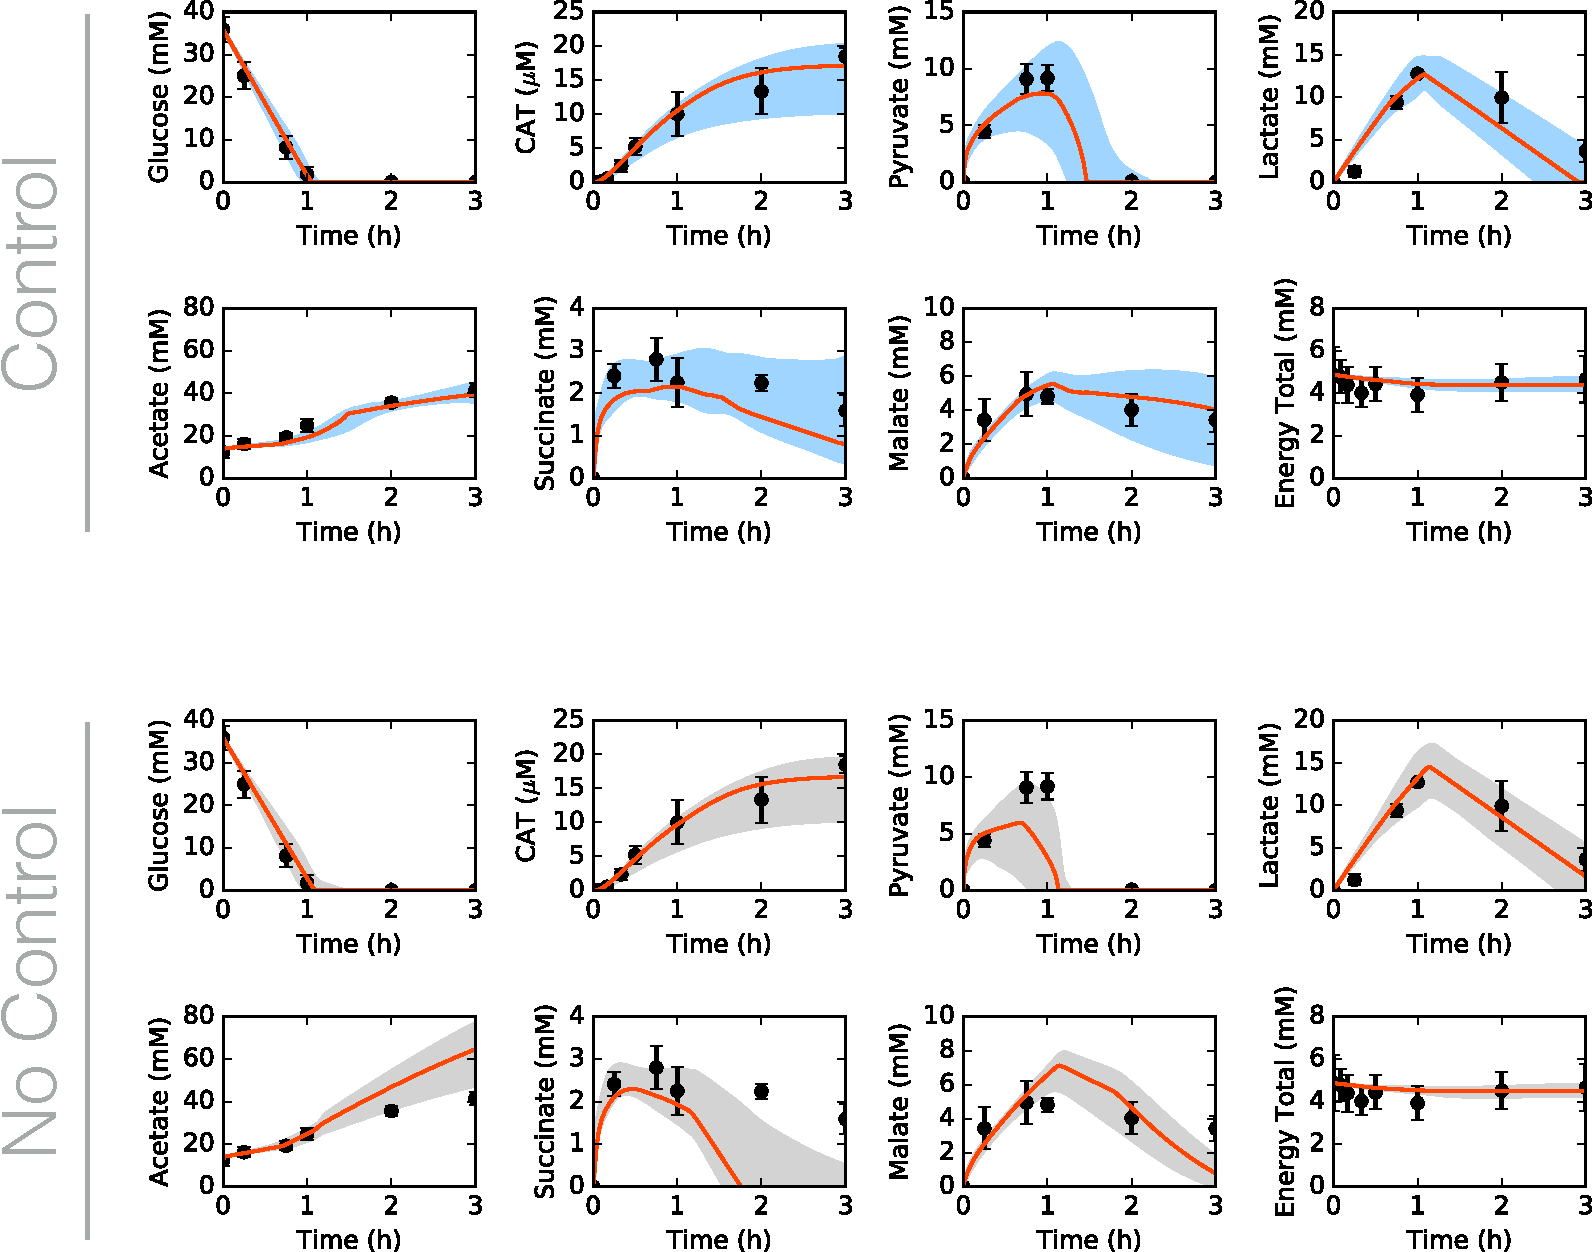
\includegraphics[width=1.00\textwidth]{./Figures/Fig_1_Carbon.pdf}
\caption{Central carbon metabolism in the presence (top) and absence (bottom) of allosteric control, including glucose (substrate), CAT (product), and intermediates, as well as total concentration of energy species. Best-fit parameter set (orange line) versus experimental data (points). 95\% confidence interval (blue or gray shaded region) over the ensemble of 100 sets.}
\label{fig:Carbon}
\end{figure}

\begin{figure}[ht]
\centering
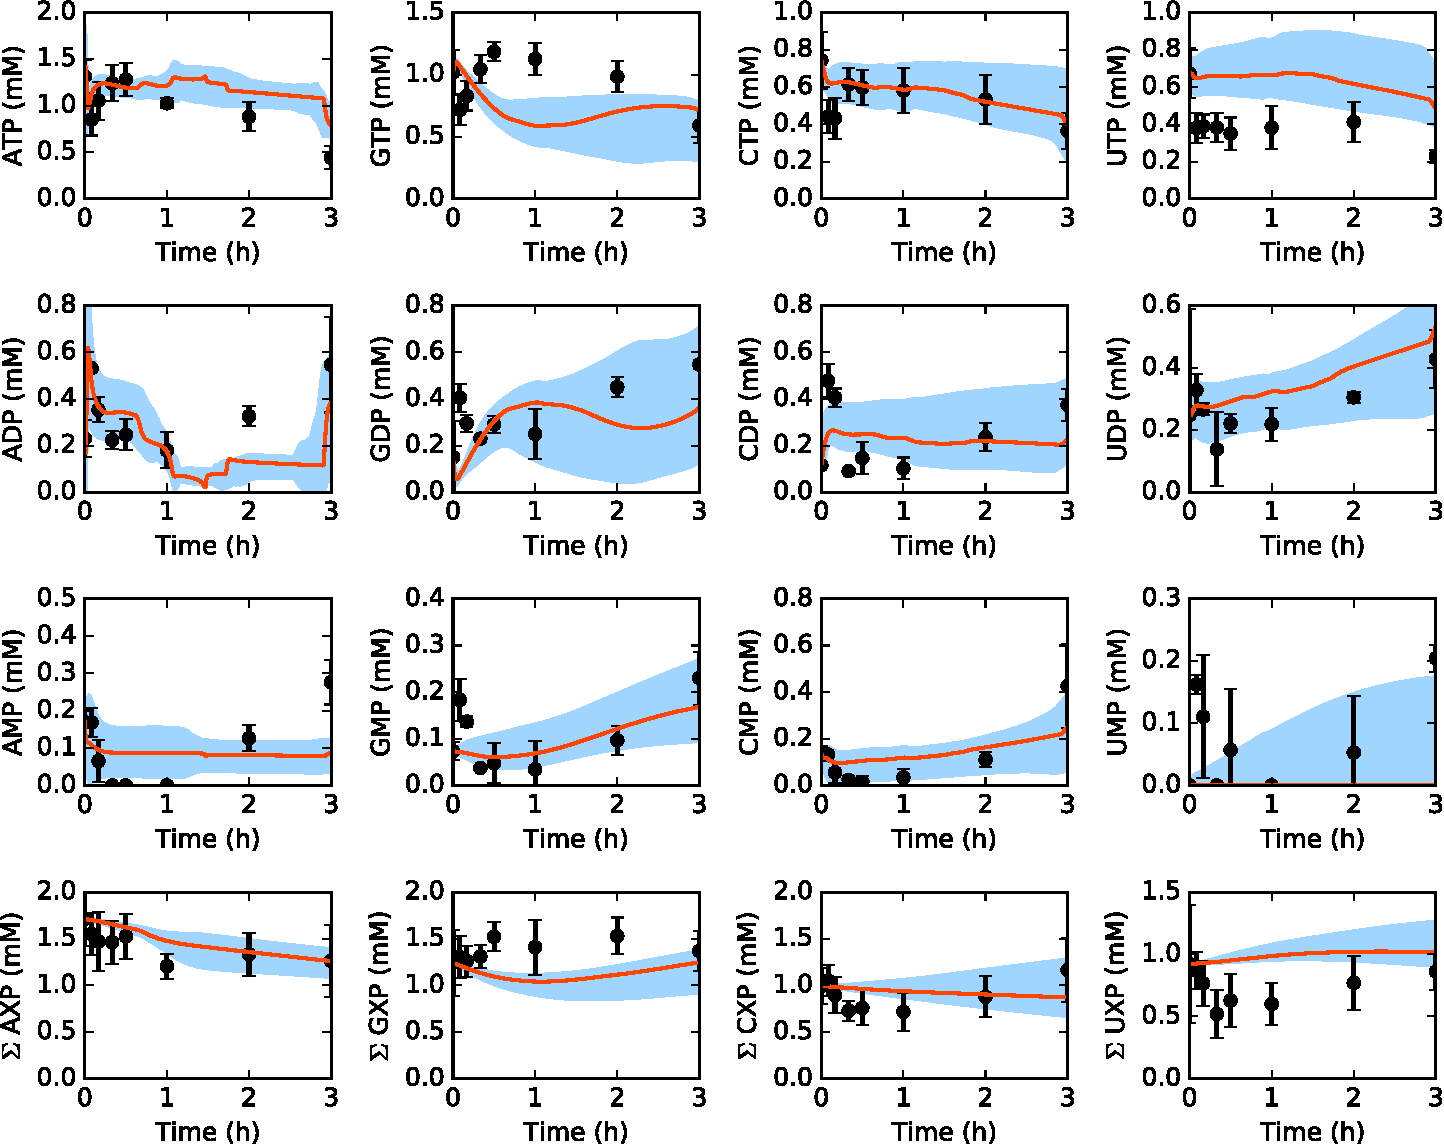
\includegraphics[width=1.00\textwidth]{./Figures/Fig_2_Energy.pdf}
\caption{Energy species and energy totals by base in the presence of allosteric control. Best-fit parameter set (orange line) versus experimental data (points). 95\% confidence interval (blue shaded region) over the ensemble of 100 sets.}
\label{fig:Energy}
\end{figure}

\begin{figure}[ht]
\centering
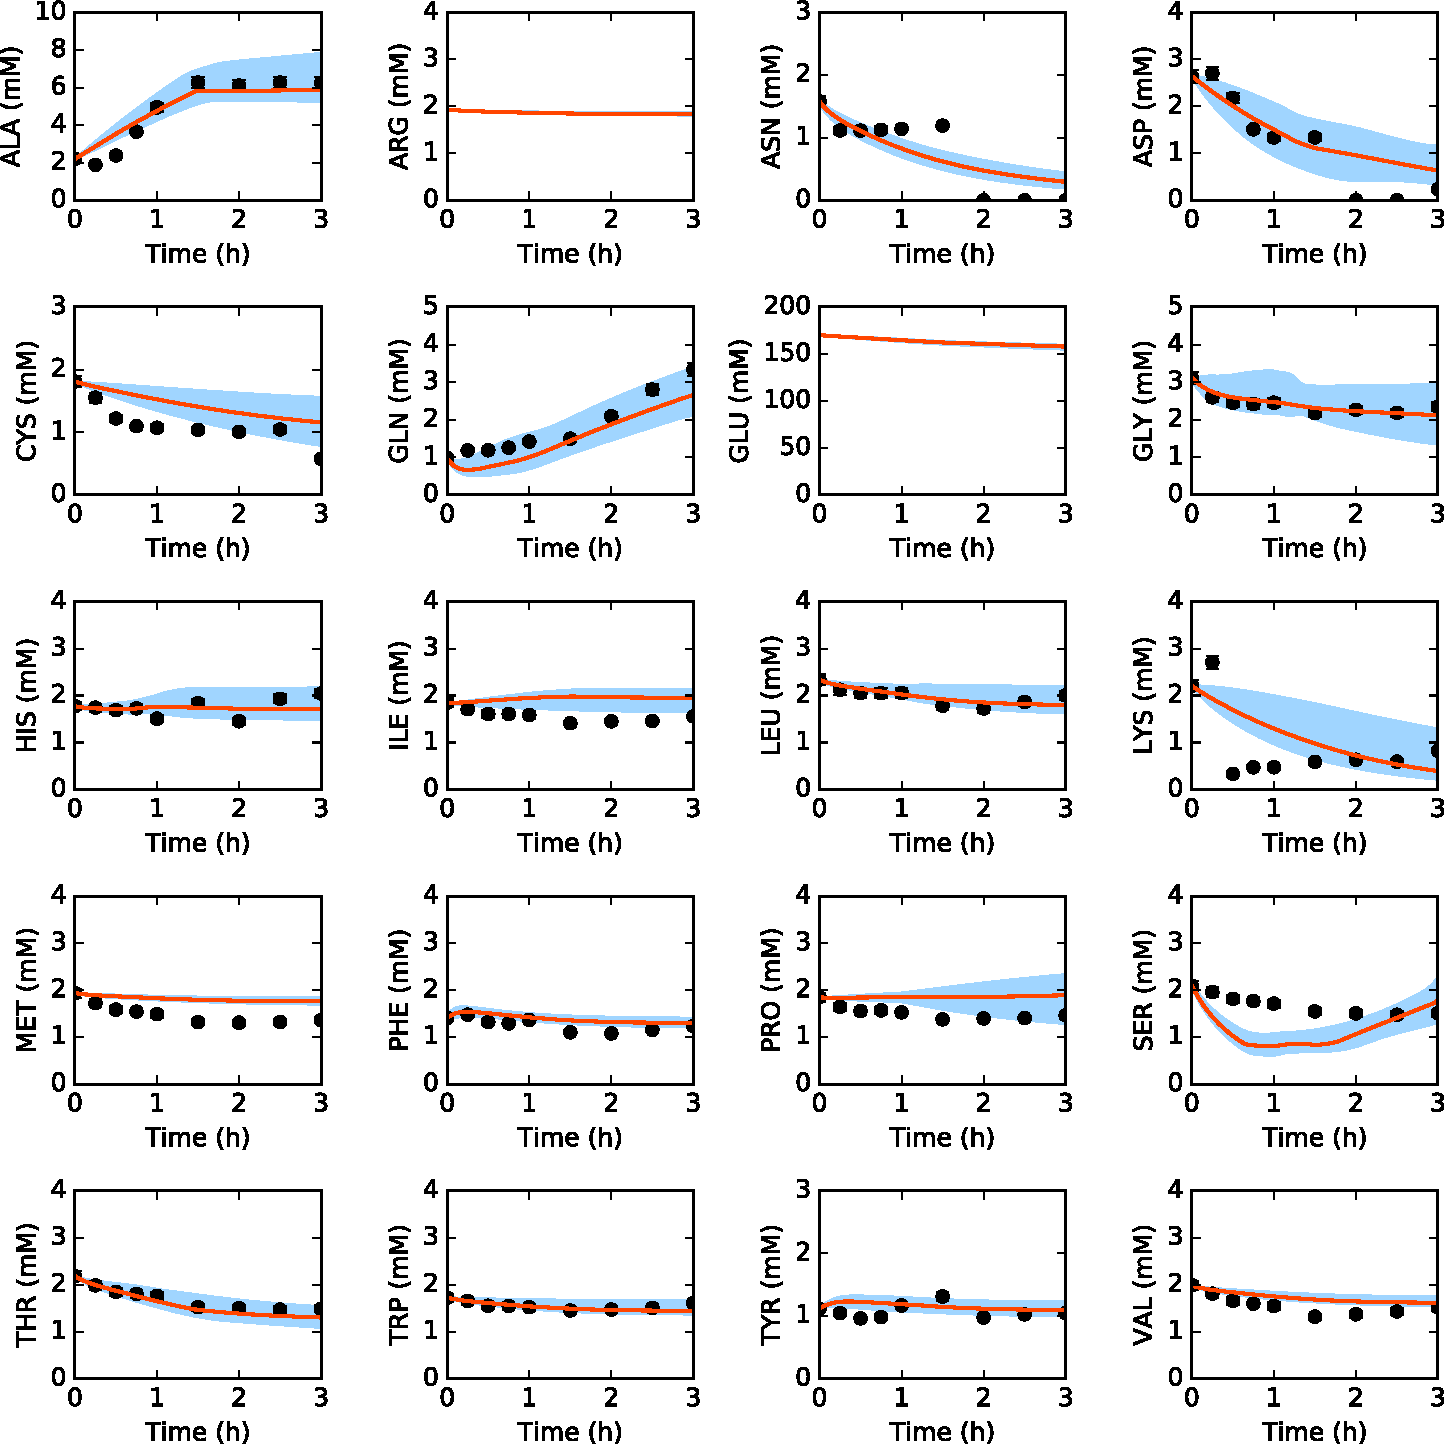
\includegraphics[width=1.00\textwidth]{./Figures/Fig_3_Amino.pdf}
\caption{Amino acids in the presence of allosteric control. Best-fit parameter set (orange line) versus experimental data (points). 95\% confidence interval (blue shaded region) over the ensemble of 100 sets.}
\label{fig:Amino}
\end{figure}

\begin{figure}[ht]
\centering
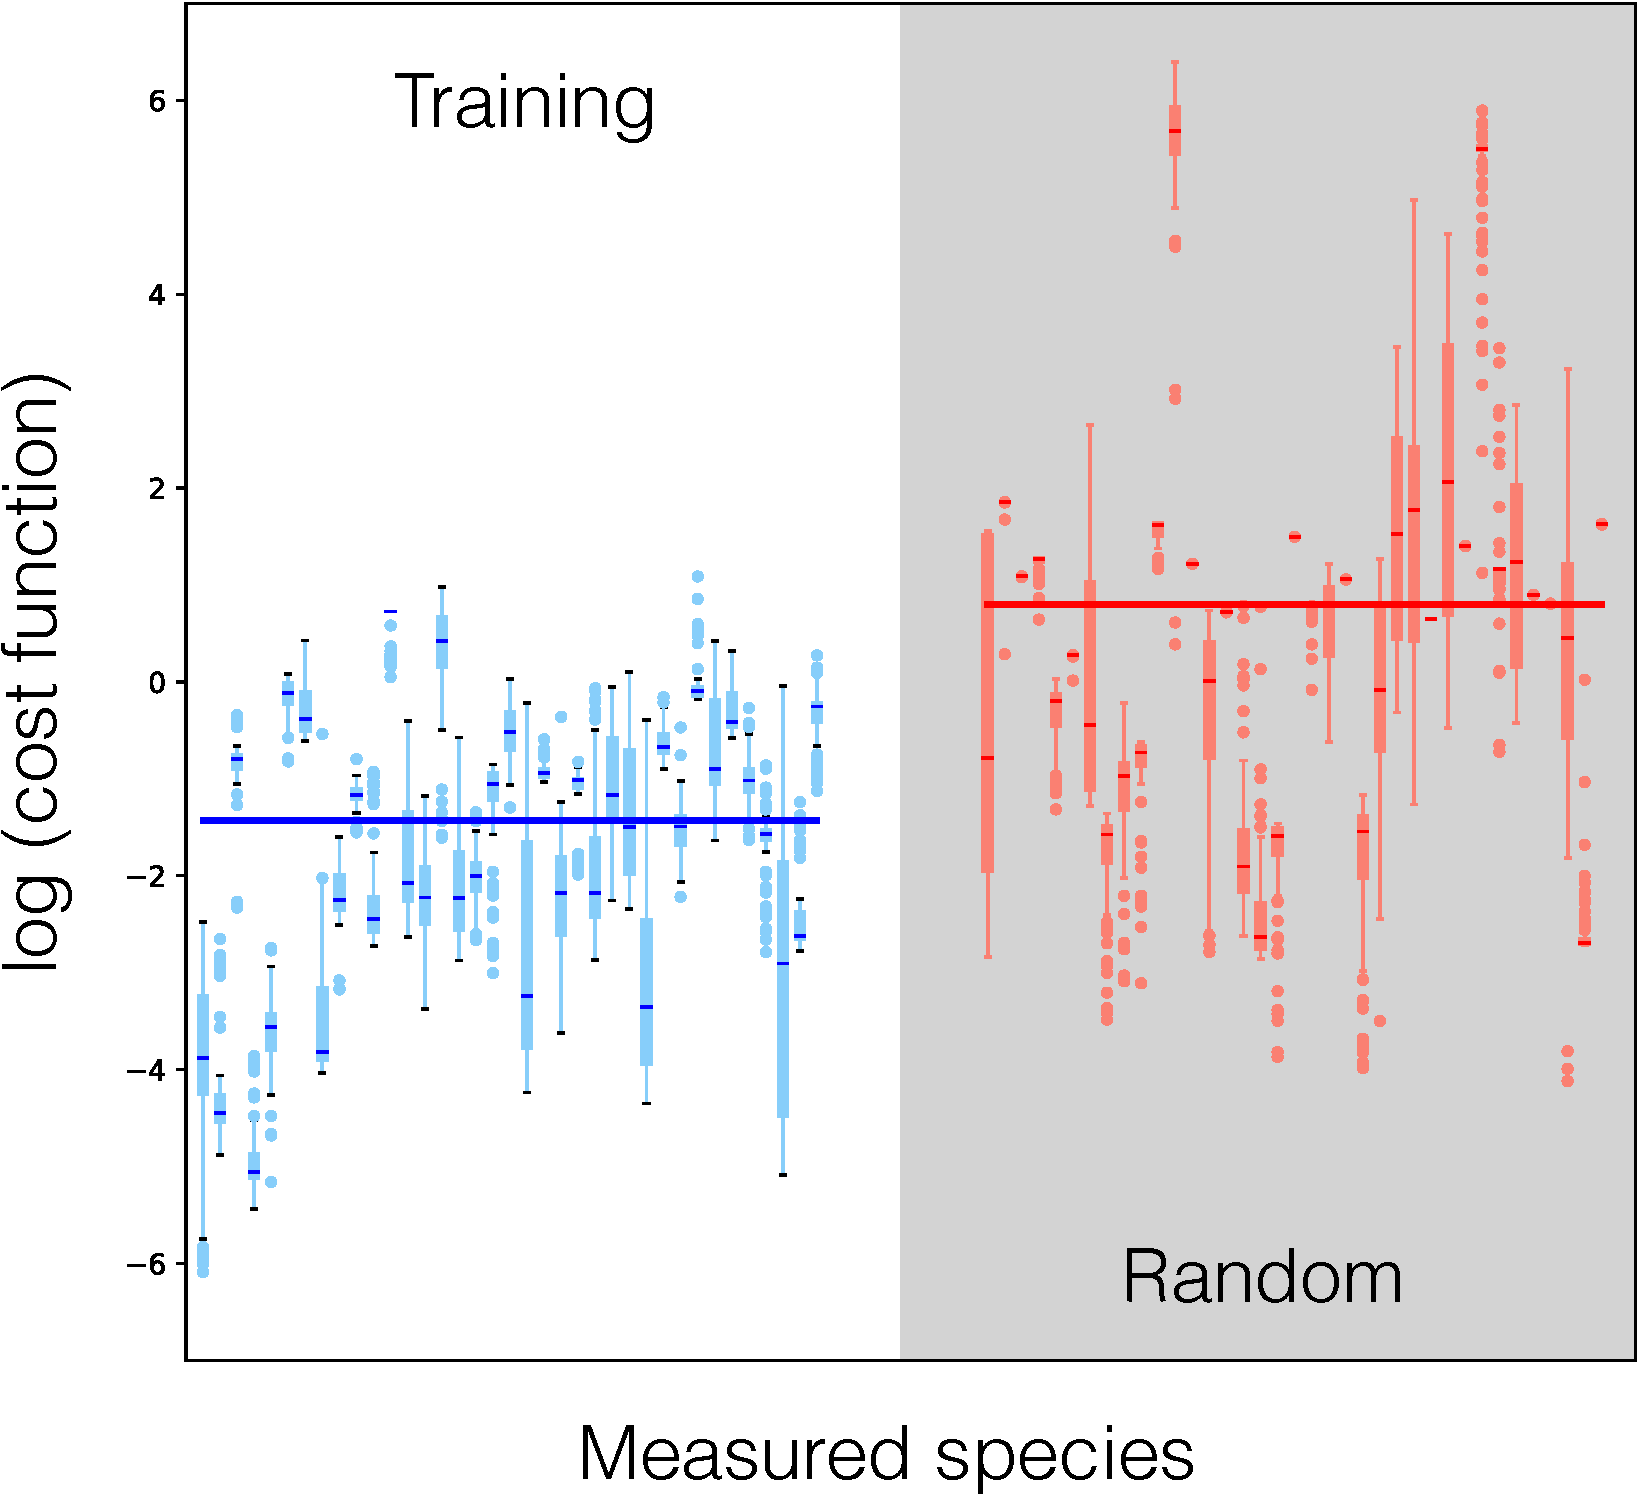
\includegraphics[width=1.00\textwidth]{./Figures/Fig_4_EnsembleVsRandom.pdf}
\caption{Log of cost function across 37 datasets for data-trained ensemble (blue) and randomly generated ensemble (red, gray background). Median (bars), interquartile range (boxes), range excluding outliers (dashed lines), and outliers (circles) for each dataset. Median across all datasets (large bar overlaid).}
\label{fig:BoxPlot}
\end{figure}

\begin{figure}[ht]
\centering
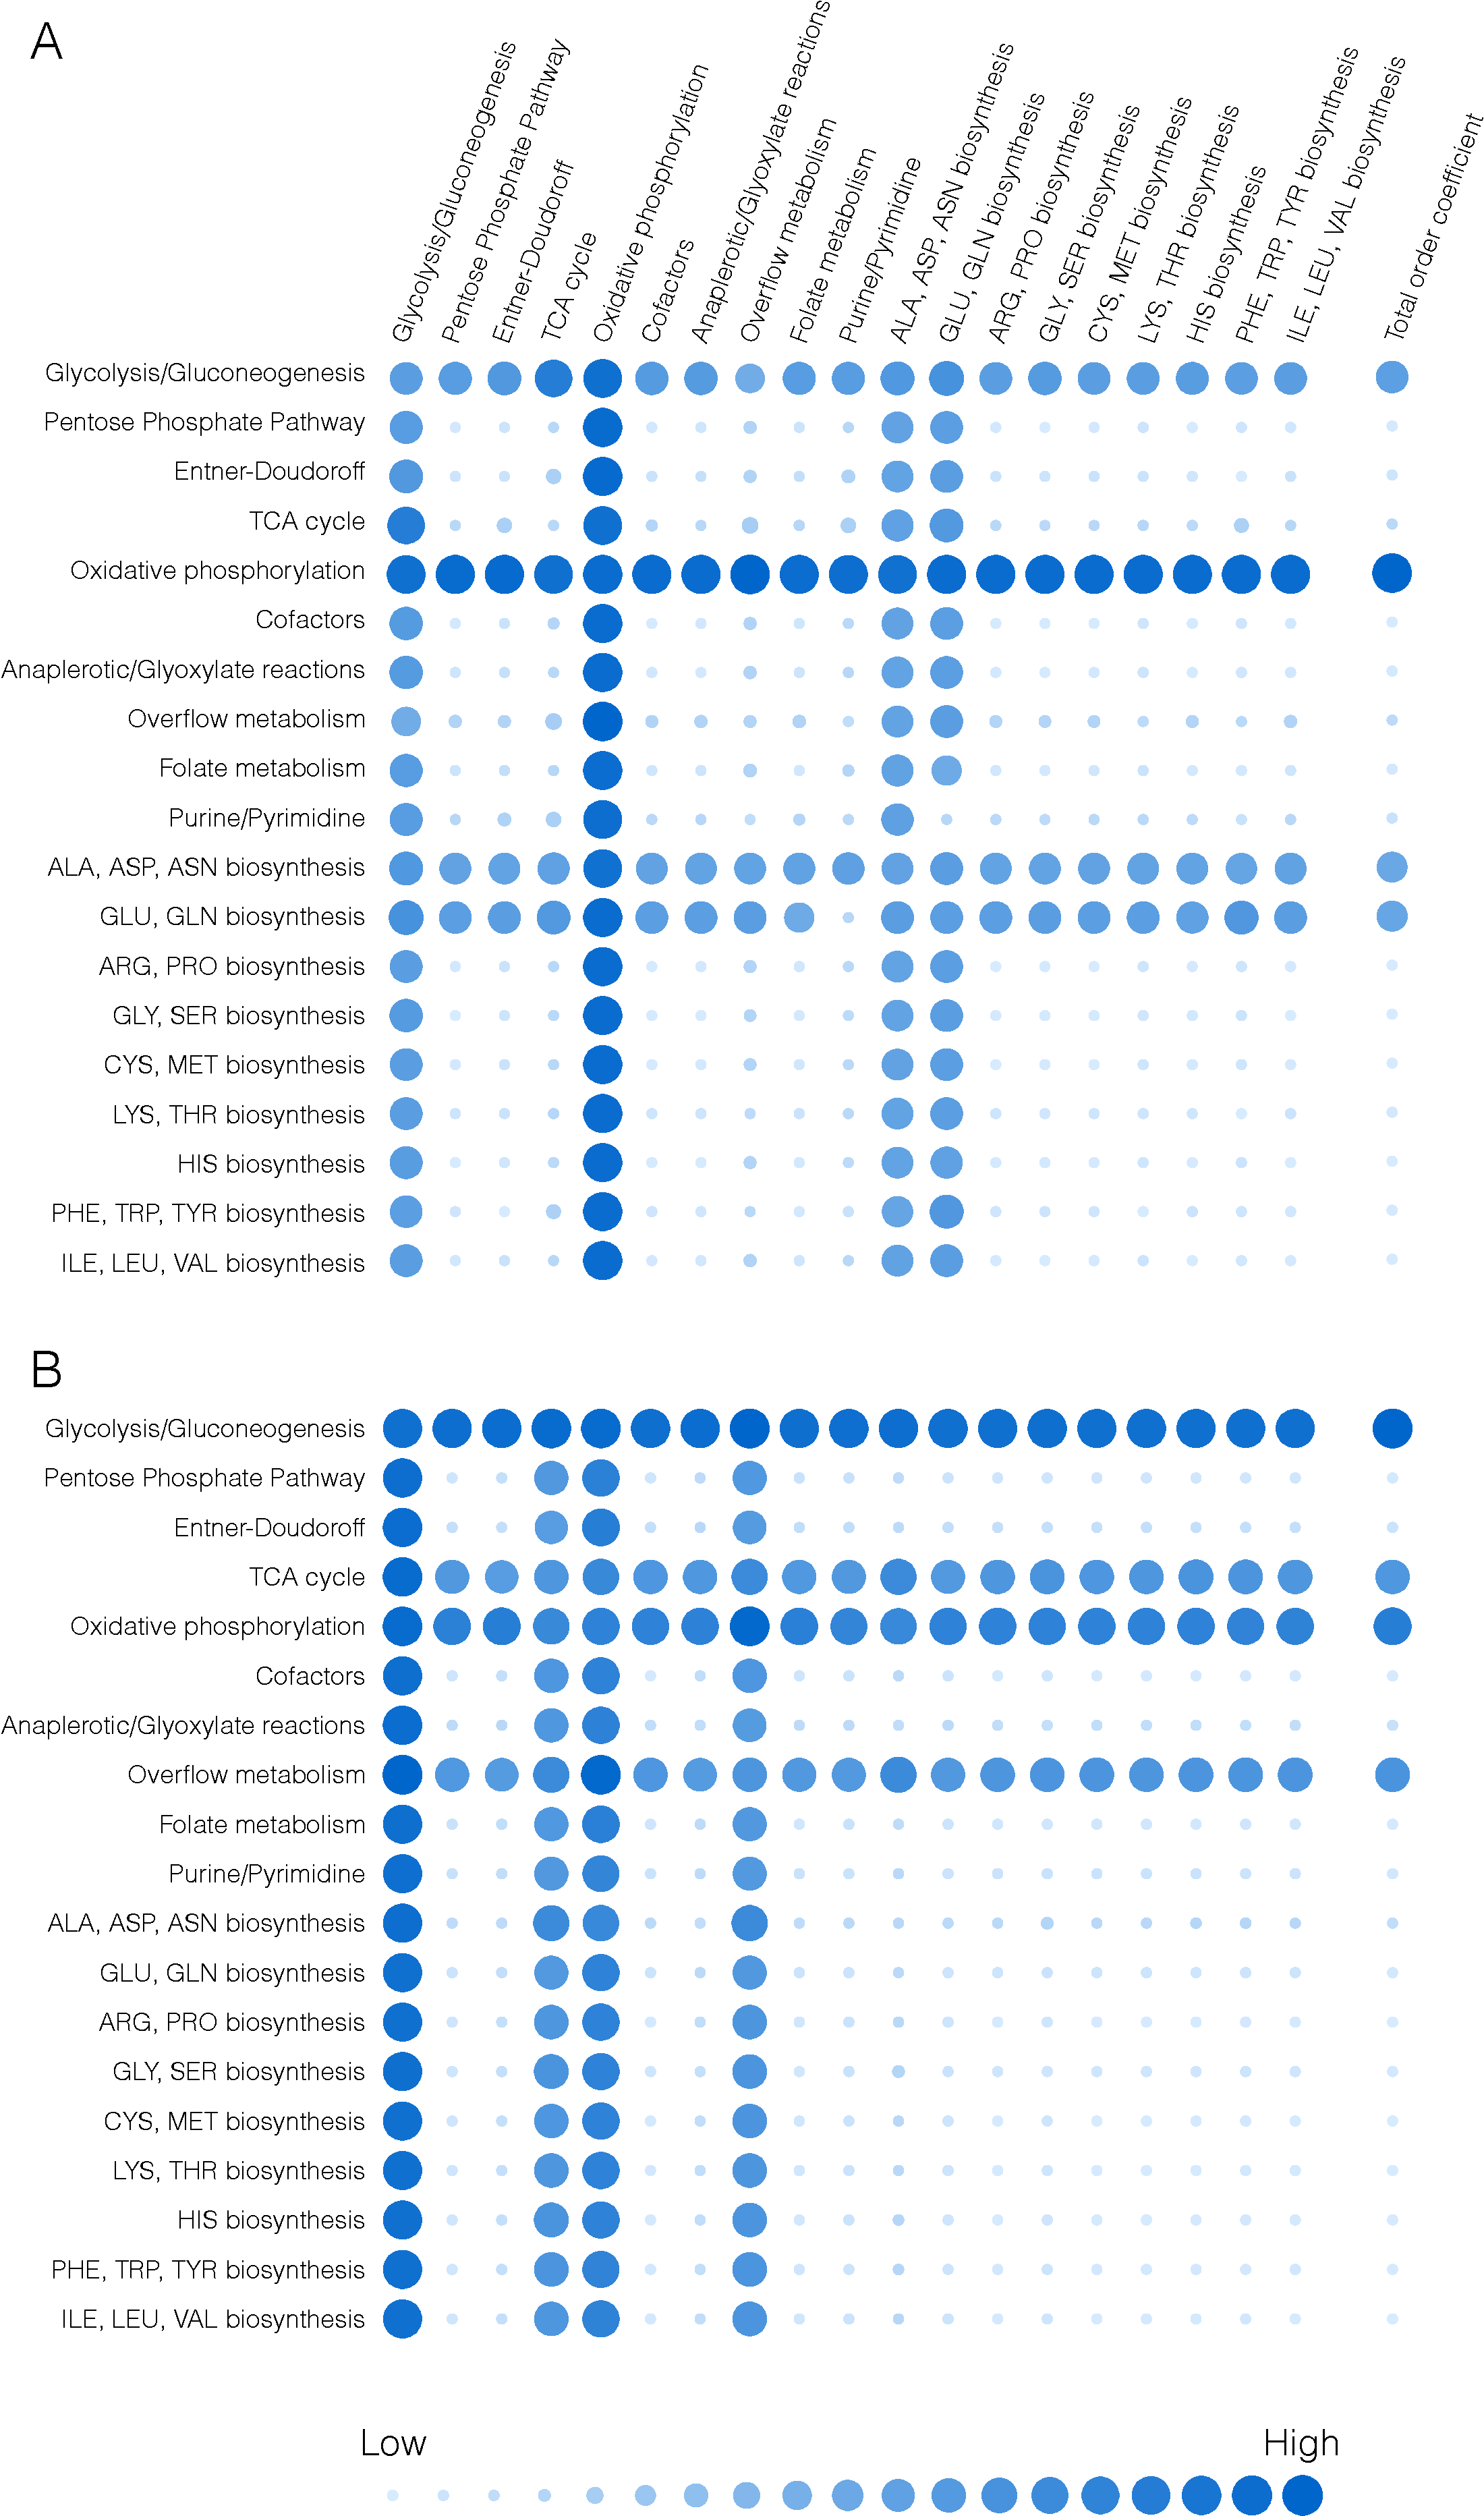
\includegraphics[width=0.7\textwidth]{./Figures/Fig_5_GroupKO.pdf}
\caption{Effect of group knockouts on system. A. Change in CAT productivity when one (diagonal) or two (off-diagonal) reaction groups are turned off. B. Change in system state (only species for which data exist) when one (diagonal) or two (off-diagonal) reaction groups are turned off. Total-order effect for each group calculated as the sum of first-order effect and all pairwise effects. Larger and darker circles represent greater effects.}
\label{fig:GroupKO}
\end{figure}

\clearpage

%\begin{table}
%\centering
% \caption{}
% \renewcommand{\arraystretch}{1.3}
% \begin{tabular}{llrrr} \toprule
% & \multicolumn{1}{r}{\textbf{Original value}} & \multicolumn{2}{r}{\textbf{After dilution factor}} & \textbf{Reference} \\ \hline
%\smallskip
%\rule{0pt}{3ex} \parbox{4.3 cm}{Characteristic Enzyme Concentration} & \multicolumn{1}{r}{5 $\mu$M} & \multicolumn{2}{r}{0.1667 $\mu$M} & 100735 \\ \toprule
%\phantom{i}\textbf{Enzyme} & \textbf{Reaction name} & \textbf{Kcat (h$^-1$)} & 
% \textbf{Vmax (mM/h)} & \textbf{Reference} \\ \hline
%\phantom{i}Serine dehydrase & R\_ser\_deg & 624000 & 104 & 101119 \\ \hline
%\phantom{i}Isocitrate dehydrogenase & R\_icd & 714000 & 119 & 101152 \\ \hline
%\phantom{i}Lactate dehydrogenase & R\_ldh & 348000 & 58 & 101036 \\ \hline
%\phantom{i}Aspartate transaminase & R\_aspC, R\_tyr, R\_phe & 1548000 & 258 & 101108 \\ \hline
%\phantom{i}Enolase & R\_eno & 792000 & 132 & 101028 \\ \hline
%\smallskip
%\rule{0pt}{3ex}
%Pyruvate kinase & R\_pyk & 1500000 & 250 & \parbox{1.4 cm}{101029, 101030} \\ \hline
%\phantom{i}Malic enzyme & R\_maeA, R\_maeB & 2124000 & 354 & 101167 \\ \hline
%\phantom{i}Phosphofructokinase & R\_pfk & 33264000 & 5544 & 104955 \\ \hline
%\phantom{i}Malate dehydrogenase & R\_mdh & 1980000 & 330 & 101163 \\ \hline
%\phantom{i}Citrate Synthase & R\_gltA & 2520000 & 420 & 101149 \\ \hline
%\phantom{i}6PG dehydrogenase & R\_zwf, R\_pgl, R\_gnd & 192000 & 32 & 101048 \\ \hline
%\phantom{i}Succinate dehydrogenase & R\_sdh & 7260 & 1.21 & 101162 \\ \hline
%\phantom{i}Succinyl-coA Synthetase & R\_sucCD & 282000 & 47 & 101158 \\ \hline
%\phantom{i}3PGA dehydrogenase & R\_gpm & 66000 & 11 & 101135 \\ \hline
%\phantom{i}PEP carboxylase & R\_ppc & 2124000 & 354 & 101139 \\ \hline
%\phantom{i}3PGA kinase & R\_pgk & 258000 & 43 & 101016 \\ \midrule
%\phantom{i}Geometric mean & & & 110 & \\ \toprule
%\phantom{i}\textbf{Transcription\slash Translation} & \textbf{AA-tRNA complex (mM)} & \textbf{Kcat (h$^-1$)} & \textbf{Vmax (mM/h)} & \textbf{Reference} \\ \hline
%\phantom{i}tRNA charging & 0.03 & 14040 & 4212 & 104980 \\ \hline
%% Serine dehydrase & Yield & 8.1\% & 6.9\% & 2.6\% \\ \bottomrule
% \end{tabular}
%\label{tbl:Rate_maxima}
%\end{table}

\begin{table}
\centering
 \caption{Reference values for reaction rate maxima (V$_{max}$) from literature. V$_{max}$ values calculated from turnover numbers (K$_{cat}$) from literature, and a characteristic enzyme concentration of 167 nM. Characteristic rate maximum for all other reactions calculated as geometric mean of calculated rate maxima.}
 \renewcommand{\arraystretch}{1.3}
 \begin{tabular}{llrrr} \toprule
\phantom{i}\textbf{Enzyme} & \textbf{Reaction} & \textbf{K$_{cat}$ (min$^{-1}$)} & 
 \textbf{V$_{max}$ (mM/h)} & \textbf{BNID \#} \\ \hline
\phantom{i}Serine dehydrase & R\_ser\_deg & 10400 & 104 & 101119 \\ \hline
\phantom{i}Isocitrate dehydrogenase & R\_icd & 11900 & 119 & 101152 \\ \hline
\phantom{i}Lactate dehydrogenase & R\_ldh & 5800 & 58 & 101036 \\ \hline
\smallskip
\rule{0pt}{4.5ex}
Aspartate transaminase & \parbox{1 cm}{R\_aspC, R\_tyr, R\_phe} & 25800 & 258 & 101108 \\ \hline
\phantom{i}Enolase & R\_eno & 13200 & 132 & 101028 \\ \hline
\smallskip
\rule{0pt}{3ex}
Pyruvate kinase & R\_pyk & 25000 & 250 & \parbox{1.4 cm}{101029 101030} \\ \hline
\smallskip
\rule{0pt}{3ex}
Malic enzyme & \parbox{1 cm}{R\_maeA, R\_maeB} & 35400 & 354 & 101167 \\ \hline
\phantom{i}Phosphofructokinase & R\_pfk & 554400 & 5544 & 104955 \\ \hline
\phantom{i}Malate dehydrogenase & R\_mdh & 33000 & 330 & 101163 \\ \hline
\phantom{i}Citrate Synthase & R\_gltA & 42000 & 420 & 101149 \\ \hline
\smallskip
\rule{0pt}{4.5ex}
6PG dehydrogenase & \parbox{1 cm}{R\_zwf, R\_pgl, R\_gnd} &3200 & 32 & 101048 \\ \hline
\phantom{i}Succinate dehydrogenase & R\_sdh & 121 & 1.21 & 101162 \\ \hline
\phantom{i}Succinyl-coA synthetase & R\_sucCD & 4700 & 47 & 101158 \\ \hline
\phantom{i}3PGA dehydrogenase & R\_gpm & 1100 & 11 & 101135 \\ \hline
\phantom{i}PEP carboxylase & R\_ppc & 35400 & 354 & 101139 \\ \hline
\phantom{i}3PGA kinase & R\_pgk & 4300 & 43 & 101016 \\ \hline
\phantom{i}Characteristic rate maximum & & & 110 & \\ \bottomrule
 \end{tabular}
\label{tbl:Rate_maxima}
\end{table}

%\begin{table}
%\centering
% \caption{}
% \renewcommand{\arraystretch}{1.3}
% \begin{tabular}{lrr} \toprule
%& \textbf{Volume (L)} & \textbf{Reference} \\ \hline
%\phantom{i}Cellular volume & 3.881e-16 & XX \\ \hline
% \toprule
% & \textbf{Concentration (mM)} & \textbf{Reference} \\ \hline
%\phantom{i}CAT gene & 5.19e-6 & XX \\ \hline
%\phantom{i}RNA polymerase & 6.75e-5 & \cite{Garamella:2016aa} \\ \hline
%\phantom{i}Ribosome & 2e-3 & \cite{Garamella:2016aa} \\ \hline
%\phantom{i}tRNA & 1.6 & 108611 \\ \hline
%\phantom{i}NAD & 1.47 & XX \\ \hline
%\phantom{i}NADH & 0.1 & XX \\ \hline
%\phantom{i}NADP & 0.195 & XX \\ \hline
%\phantom{i}NADPH & 0.062 & XX \\ \hline
%\phantom{i}G6P & 3.48 & XX \\ \hline
%\phantom{i}F6P & 0.6 & XX \\ \hline
%\phantom{i}FDP & 0.272 & XX \\ \hline
%\phantom{i}DHAP & 0.167 & XX \\ \hline
%\phantom{i}G3P & 0.218 & XX \\ \hline
%\phantom{i}13DPG & 0.008 & XX \\ \hline
%\phantom{i}3PG & 2.13 & XX \\ \hline
%\phantom{i}2PG & 0.399 & XX \\ \hline
%\phantom{i}6PGL & 0.808 & XX \\ \hline
%\phantom{i}6PGC & 0.808 & XX \\ \hline
%\phantom{i}RU5P & 0.111 & XX \\ \hline
%\phantom{i}XU5P & 0.138 & XX \\ \hline
%\phantom{i}R5P & 0.398 & XX \\ \hline
%\phantom{i}S7P & 0.276 & XX \\ \hline
%\phantom{i}E4P & 0.098 & XX \\ \hline
%\phantom{i}NH3 & 0.052425 & XX \\ \hline
%\phantom{i}ARG & 1.9326 & XX \\ \hline
%\phantom{i}H2O2 & 0.052425 & XX \\ \hline
%\phantom{i}HCO3 & 0.052425 & XX \\ \hline
%% \bottomrule
% \end{tabular}
%\label{tbl:Initial_conditions}
%\end{table}

%\begin{table}
%\centering
% \caption{}
% \renewcommand{\arraystretch}{1.3}
% \begin{tabular}{llrrr} \toprule
% & & \textbf{Original value} & \textbf{After dilution factor} & \textbf{Reference} \\ \hline
%\smallskip
%\rule{0pt}{3ex} \parbox{4.3 cm}{Characteristic Enzyme Concentration} & & 5 $\mu$M & 0.1667 $\mu$M & 100735 \\ \toprule
%\phantom{i}\textbf{Enzyme} & \textbf{Reaction} & \textbf{Kcat (h$^-1$)} & 
% \textbf{Vmax (mM/h)} & \textbf{Reference} \\ \hline
%\phantom{i}Serine dehydrase & R\_ser\_deg & 624000 & 104 & 101119 \\ \hline
%\phantom{i}Isocitrate dehydrogenase & R\_icd & 714000 & 119 & 101152 \\ \hline
%\phantom{i}Lactate dehydrogenase & R\_ldh & 348000 & 58 & 101036 \\ \hline
%\smallskip
%\rule{0pt}{4.5ex}
%Aspartate transaminase & \parbox{1 cm}{R\_aspC, R\_tyr, R\_phe} & 1548000 & 258 & 101108 \\ \hline
%\phantom{i}Enolase & R\_eno & 792000 & 132 & 101028 \\ \hline
%\smallskip
%\rule{0pt}{3ex}
%Pyruvate kinase & R\_pyk & 1500000 & 250 & \parbox{1.4 cm}{101029, 101030} \\ \hline
%\smallskip
%\rule{0pt}{3ex}
%Malic enzyme & \parbox{1 cm}{R\_maeA, R\_maeB} & 2124000 & 354 & 101167 \\ \hline
%\phantom{i}Phosphofructokinase & R\_pfk & 33264000 & 5544 & 104955 \\ \hline
%\phantom{i}Malate dehydrogenase & R\_mdh & 1980000 & 330 & 101163 \\ \hline
%\phantom{i}Citrate Synthase & R\_gltA & 2520000 & 420 & 101149 \\ \hline
%\smallskip
%\rule{0pt}{4.5ex}
%6PG dehydrogenase & \parbox{1 cm}{R\_zwf, R\_pgl, R\_gnd} & 192000 & 32 & 101048 \\ \hline
%\phantom{i}Succinate dehydrogenase & R\_sdh & 7260 & 1.21 & 101162 \\ \hline
%\phantom{i}Succinyl-coA synthetase & R\_sucCD & 282000 & 47 & 101158 \\ \hline
%\phantom{i}3PGA dehydrogenase & R\_gpm & 66000 & 11 & 101135 \\ \hline
%\phantom{i}PEP carboxylase & R\_ppc & 2124000 & 354 & 101139 \\ \hline
%\phantom{i}3PGA kinase & R\_pgk & 258000 & 43 & 101016 \\ \midrule
%\phantom{i}Geometric mean & & & 110 & \\ \toprule
%%\phantom{i}\textbf{Transcription\slash Translation} & \textbf{AA-tRNA (mM)} & \textbf{Kcat (h$^-1$)} & \textbf{Vmax (mM/h)} & \textbf{Reference} \\ \hline
%\phantom{i}tRNA charging & 0.03 & 14040 & 4212 & 104980 \\ \hline
%% \bottomrule
% \end{tabular}
%\label{tbl:Rate_maxima}
%\end{table}

%\begin{table}
%\centering
%    \caption{CAT carbon yield breakdown for best-fit set, knockouts, and experimental data. Carbon produced as CAT, carbon consumed as glucose and each amino acid, sum of consumed species, and yield. Accumulation of alanine and glutamine (negative consumption terms) was not considered in yield calculation.}
%    \renewcommand{\arraystretch}{1.3}
%    \begin{tabular}{lrrrrrr} \toprule
%        Carbon Produced (C-mM) & Best-fit & $\Delta$app & $\Delta$nuo & $\Delta$cyd & \parbox{1 cm}{$\Delta$app $\Delta$nuo $\Delta$cyd} & Data \\ \hline
%        CAT & 20.9 & 21.4 & 18.1 & 6.5 & 5.1 & 21.6 \\ \midrule
%        Carbon Consumed (C-mM) \\ \hline
%        GLC & 215.4 & 215.4 & 215.4 & 215.4 & 159.8 & 215.4 \\ \hline
%        ALA & -11.6 & -11.4 & 1.7 & -3.8 & -3.2 & -12.1 \\ \hline
%%        ARG & 10.2 & 9.9 & 1.1 & 0.9 & 1.3 & - \\ \hline
%        ASN & 6.2 & 6.2 & 6.2 & 6.3 & 6.3 & 6.3 \\ \hline
%        ASP & 7.5 & 7.5 & 3.9 & 0.0 & 0.0 & 9.6 \\ \hline
%        CYS & 3.0 & 3.1 & 3.0 & 2.9 & 2.9 & 3.7 \\ \hline
%        GLN & -11.4 & -11.3 & -4.0 & 1.8 & 2.7 & -11.7 \\ \hline
%%        GLU & 492.6 & 505.6 & 528.2 & 505.1 & 501.8 & - \\ \hline
%        GLY & 3.1 & 3.1 & 2.6 & 1.1 & 0.9 & 1.5 \\ \hline
%        HIS & 0.2 & 0.2 & 1.1 & 0.4 & 0.3 & 0.0 \\ \hline
%        ILE & 1.0 & 1.0 & 0.8 & 0.3 & 0.2 & 1.7 \\ \hline
%        LEU & 1.4 & 1.4 & 1.2 & 0.4 & 0.3 & 2.0 \\ \hline
%        LYS & 10.7 & 10.7 & 13.1 & 13.2 & 13.2 & 8.3 \\ \hline
%        MET & 0.8 & 0.8 & 0.7 & 0.2 & 0.2 & 2.9 \\ \hline
%        PHE & 3.2 & 3.3 & 2.8 & 1.0 & 0.8 & 1.6 \\ \hline
%        PRO & 2.4 & 2.4 & 0.7 & 0.2 & 0.2 & 1.9 \\ \hline
%        SER & 2.5 & 2.5 & 2.4 & 2.1 & 2.1 & 1.8 \\ \hline
%        THR & 3.4 & 3.4 & 3.3 & 2.9 & 2.8 & 2.8 \\ \hline
%        TRP & 1.0 & 1.0 & 0.8 & 0.3 & 0.2 & 1.2 \\ \hline
%        TYR & 1.1 & 1.1 & 1.1 & 0.4 & 0.4 & 0.6 \\ \hline
%        VAL & 1.4 & 1.5 & 1.2 & 0.4 & 0.4 & 2.4 \\ \midrule
%%        Sum & 767.1 & 780.1 & 791.3 & 755.3 & 696.8 & - \\ \hline
%        Sum & 264.3 & 264.6 & 262.0 & 249.3 & 193.7 & 263.7 \\ \midrule
%%        Yield & 2.7\% & 2.7\% & 2.3\% & 0.9\% & 0.7\% & - \\ \hline
%        Yield & 7.9\% & 8.1\% & 6.9\% & 2.6\% & 2.7\% & 8.2\% \\ \bottomrule
%    \end{tabular}
%\label{tbl:yield_breakdown}
%\end{table}

\clearpage

\begin{figure}[ht]
\centering
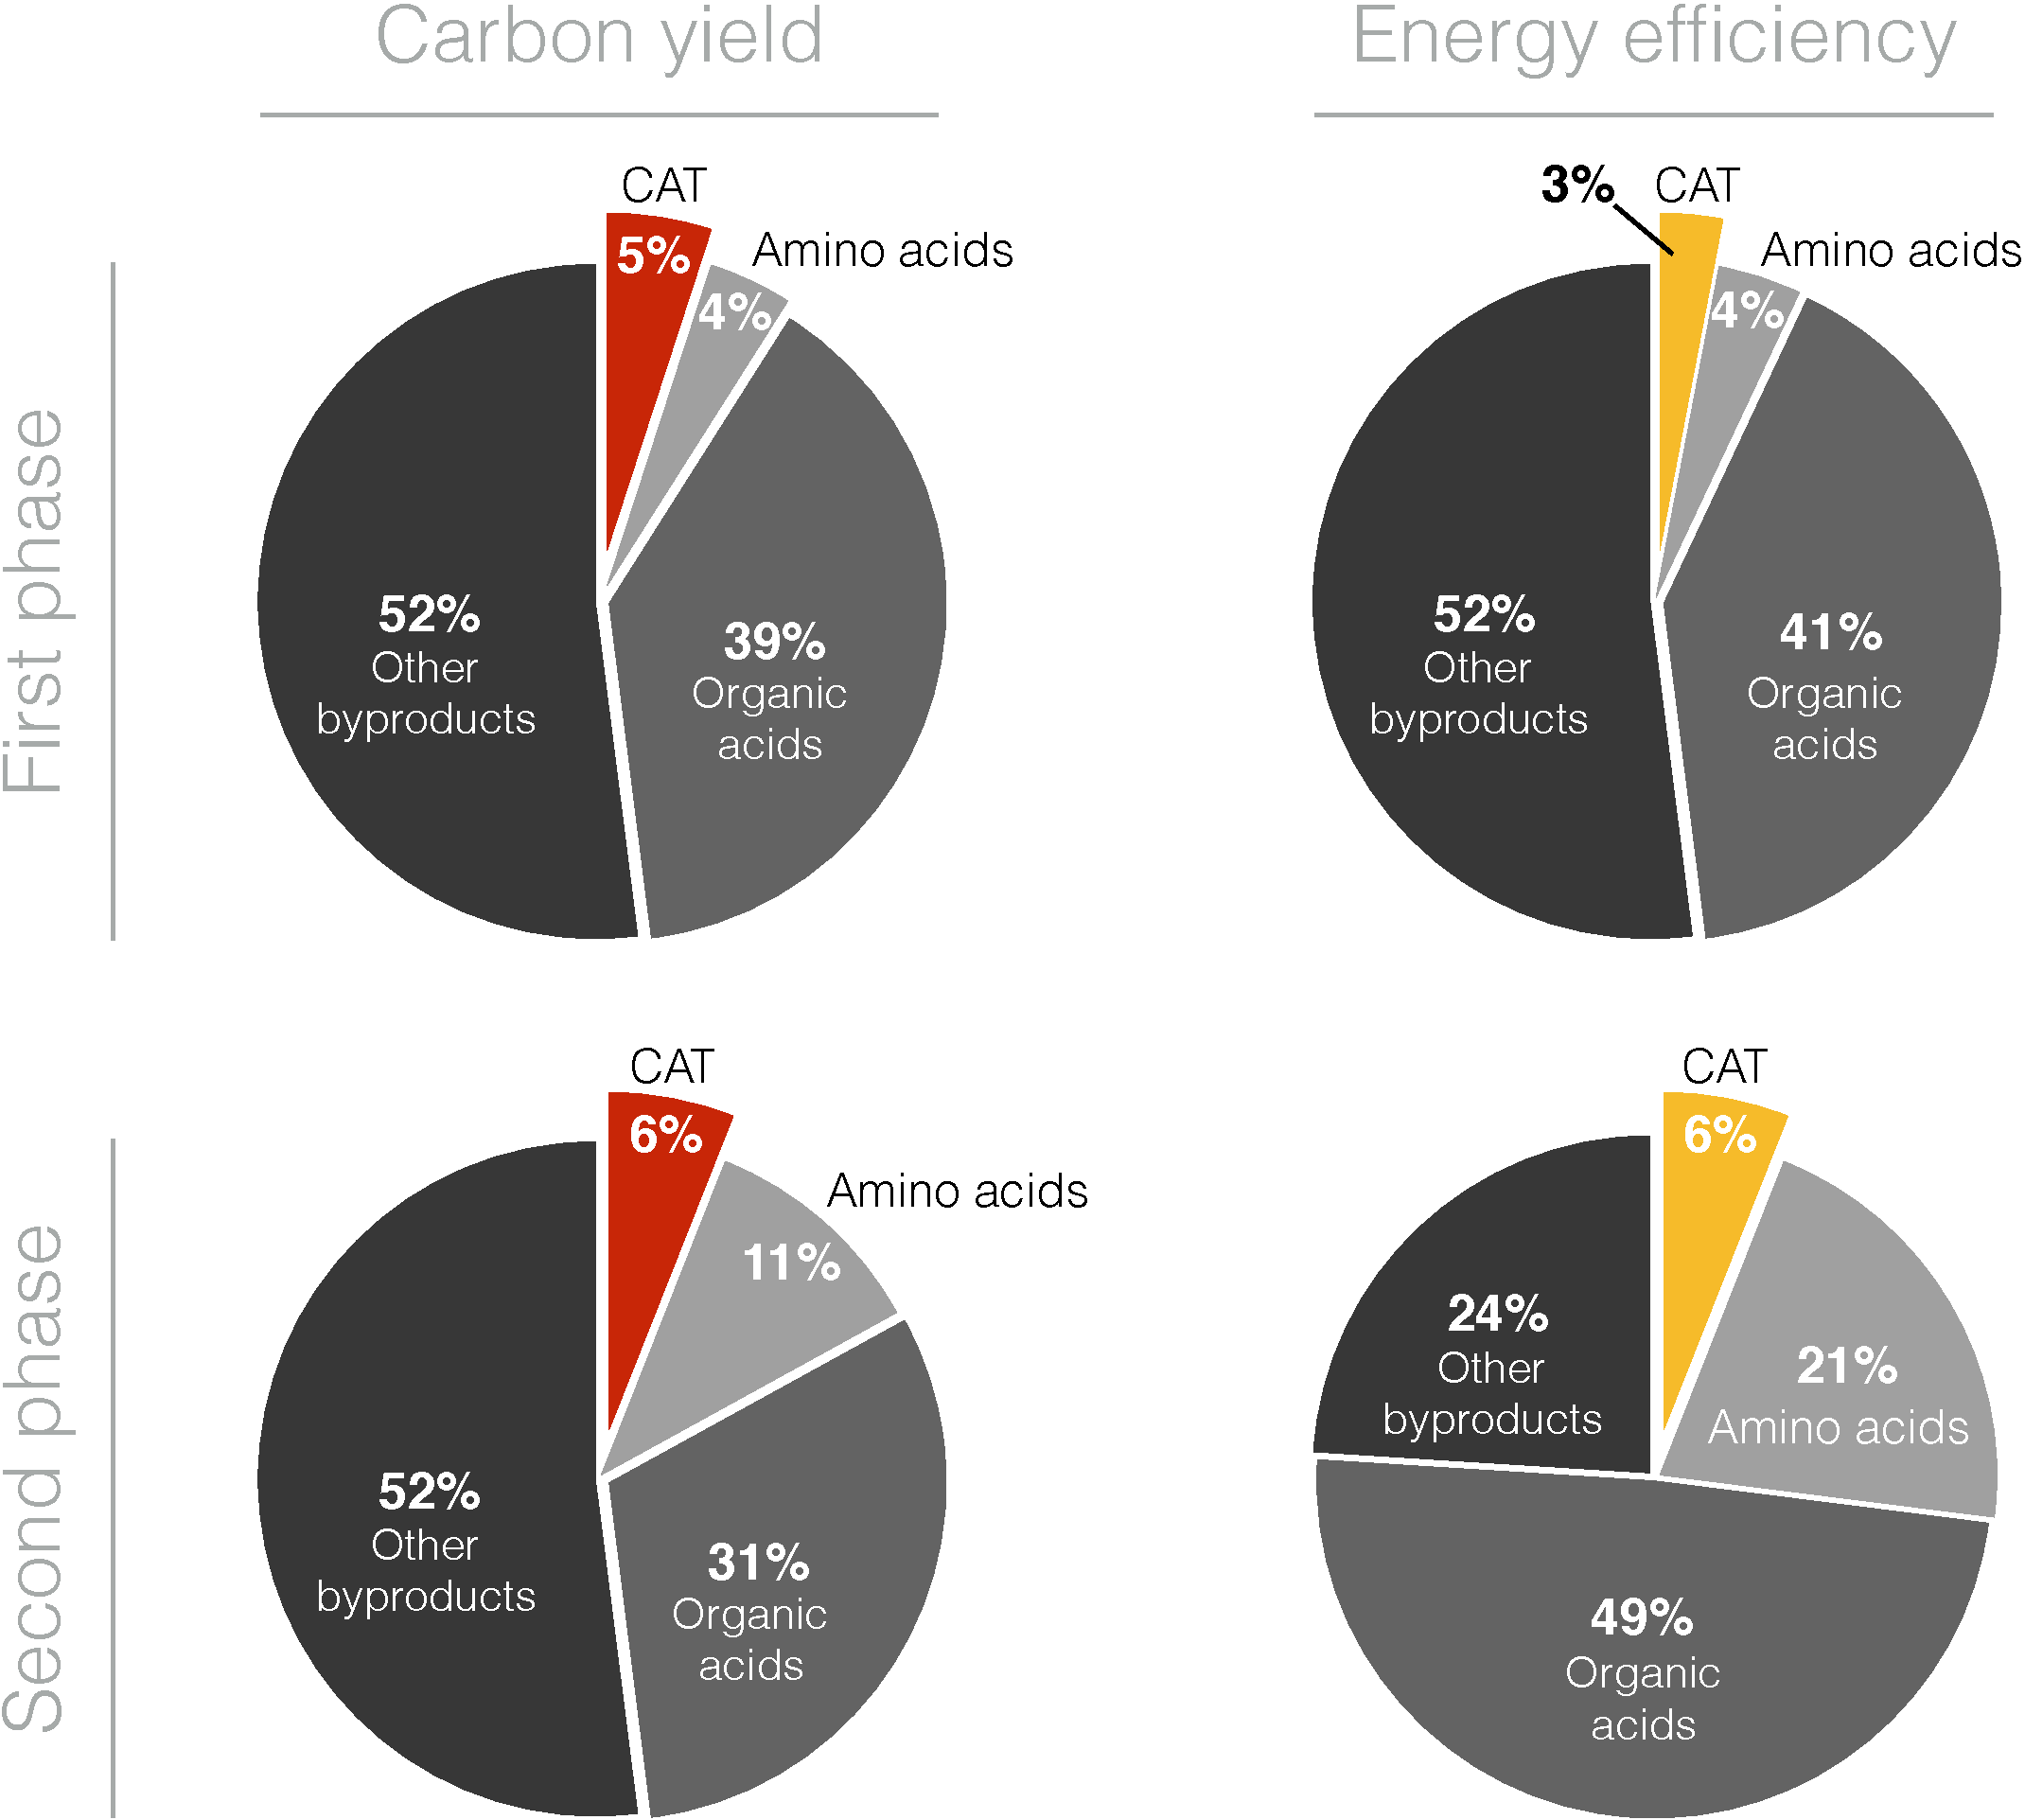
\includegraphics[width=1.00\textwidth]{./Figures/Fig_6_CarbonEnergyBalances.pdf}
%\caption{Carbon and energy balances for the best-fit set. A. Carbon moles produced as CAT, amino acids (alanine and glutamine), organic acids (lactate, acetate, succinate, and malate), and other byproducts including carbon dioxide, as percentages of total carbon consumption (glucose and all other amino acids). B. Energy cost of CAT production, accumulation of amino acids (alanine and glutamine), accumulation of organic acids (lactate, acetate, succinate, and malate), and other byproducts, as percentages of total energy utilization from glucose. Energy costs calculated in terms of equivalent ATP molecules.}
\caption{Carbon and energy balances during the first and second phases of protein production for the best-fit set. Top left: Carbon moles produced as CAT, amino acids (alanine, isoleucine, glutamine, proline, and tyrosine), organic acids (pyruvate, lactate, acetate, succinate, and malate), and all other byproducts, as percentages of total carbon consumption (glucose and all other amino acids). Bottom left: Carbon moles produced as CAT, amino acids (alanine, glutamine, proline, and serine), organic acids (acetate only), and all other byproducts, as percentages of total carbon consumption (pyruvate, lactate, succinate, malate, and all other amino acids). Top right: Energy cost of CAT production, accumulation of amino acids (alanine, isoleucine, glutamine, proline, and tyrosine), accumulation of organic acids (pyruvate, lactate, acetate, succinate, and malate), and other byproducts, as percentages of total energy utilization from glucose. Bottom right: Energy cost of CAT production, accumulation of amino acids (alanine, glutamine, proline, and serine), accumulation of organic acids (acetate only), and other byproducts, as percentages of total energy utilization from pyruvate, lactate, succinate, and malate. Energy costs calculated in terms of equivalent ATP molecules.}
% including carbon dioxide
\label{fig:CAT_balances}
\end{figure}

\clearpage

% Supplemental figures -
% Set the S-
\renewcommand\thefigure{S\arabic{figure}}
\renewcommand\thetable{T\arabic{table}}
\renewcommand\thepage{S-\arabic{page}}
\renewcommand\theequation{S\arabic{equation}}

% Reset the counters -
\setcounter{equation}{0}
\setcounter{table}{0}
\setcounter{figure}{0}
\setcounter{page}{1}

% Supplemental figures go here ...
%\begin{figure}[ht]
%\centering
%\includegraphics[width=1.00\textwidth]{./figs/<Filename>.pdf}
%\caption{Captiontext goes here}
%}\label{fig:<label_name>}
%\end{figure}

\end{document}
\grid
\grid
